
\documentclass{beamer}
\usecolortheme{dove}
\setbeamertemplate{navigation symbols}{}
\usepackage{amsmath,amssymb,amsfonts,amsthm, multicol, subfigure, color}
\setbeamertemplate{footline}[text line]{\parbox{\linewidth}{\vspace*{-8pt}\bgray{Panel Data} \insertsectionnavigationhorizontal{.75\paperwidth}{}{\hfill\hfill}}}
\usepackage{bm}
\usepackage{graphicx}
\usepackage{tabularx}
\usepackage{booktabs}
\usepackage{hyperref}
\usepackage{pdfpages}
\usepackage{xcolor}
\definecolor{seagreen}{RGB}{46, 139, 87}
\def\independenT#1#2{\mathrel{\rlap{$#1#2$}\mkern2mu{#1#2}}}
\newcommand\indep{\protect\mathpalette{\protect\independenT}{\perp}}
\def\log{\text{log}}
\newcommand\logit{\text{logit}}
\newcommand\iid{\stackrel{\text{iid}}{\sim}}
\newcommand\E{\text{E}}
\newcommand\V{\text{V}}
\renewcommand\P{\text{P}}
\newcommand{\Cov}{\text{Cov}}
\newcommand{\Cor}{\text{Cor}}
\newcommand\doop{\texttt{do}}
\usepackage{stackrel}
\usepackage{tikz}
\usetikzlibrary{arrows,shapes.arrows,positioning,shapes,patterns,calc}
\newcommand\slideref[1]{\vskip .1cm \tiny \textcolor{gray}{{#1}}}
\newcommand\red[1]{\color{red}#1}
\newcommand\blue[1]{\color{blue}#1}
\newcommand\gray[1]{\color{gray}#1}
\newcommand\seagreen[1]{\color{seagreen}#1}
\newcommand\purple[1]{\color{purple}#1}
\newcommand\orange[1]{\color{orange}#1}
\newcommand\black[1]{\color{black}#1}
\newcommand\white[1]{\color{white}#1}
\newcommand\teal[1]{\color{teal}#1}
\newcommand\magenta[1]{\color{magenta}#1}
\newcommand\Fuchsia[1]{\color{Fuchsia}#1}
\newcommand\BlueGreen[1]{\color{BlueGreen}#1}
\newcommand\bblue[1]{\textcolor{blue}{\textbf{#1}}}
\newcommand\bred[1]{\textcolor{red}{\textbf{#1}}}
\newcommand\bgray[1]{\textcolor{gray}{\textbf{#1}}}
\newcommand\bgreen[1]{\textcolor{seagreen}{\textbf{#1}}}
\newcommand\bref[2]{\href{#1}{\color{blue}{#2}}}
\colorlet{lightgray}{gray!40}
\pgfdeclarelayer{bg}    % declare background layer for tikz
\pgfsetlayers{bg,main} % order layers for tikz
\newcommand\mycite[1]{\begin{scriptsize}\textcolor{darkgray}{(#1)}\end{scriptsize}}
\newcommand{\tcframe}{\frame{
%\small{
\only<1|handout:0>{\tableofcontents}
\only<2|handout:1>{\tableofcontents[currentsubsection]}}
%}
}

\usepackage[round]{natbib}
\bibliographystyle{humannat-mod}
\setbeamertemplate{enumerate items}[default]
\usepackage{mathtools}
\usepackage{ulem}

% Need to add examples

\newcommand{\goalsframe}{\begin{frame}{Learning goals for today}
At the end of class, you will be able to:
\begin{enumerate}
\item Recognize the promises and pitfalls of four methods to study the effects of treatments that turn on once
\begin{enumerate}
\item Difference in difference (DID)
\item Interrupted time series (ITS)
\item Regression discontinuity (RD)
\item Synthetic control (SC)
\end{enumerate}
\end{enumerate} \vskip .2in
\end{frame}}

\title{Panel Data\\\vskip .1in\begin{small}Difference in difference\\Interrupted time series\\Regression discontinuity\\Synthetic control\\{}\end{small}}
\author{Ian Lundberg\\Soc 212B\\Winter 2025}
\date{5 Feb 2025}

\begin{document}

\maketitle

\goalsframe

\section{Difference in Difference}

\begin{frame}
Card, D., \& Krueger, A. B. (1994).\\\bref{https://davidcard.berkeley.edu/papers/njmin-aer.pdf}{Minimum Wages and Employment: A Case Study of the Fast-Food Industry in New Jersey and Pennsylvania.}\\The American Economic Review, 84(4), 772-793.
\end{frame}

\begin{frame}{Economic theory}
When the minimum wage rises, how might employment change? \pause
\begin{itemize}
\item employees cost more \pause
\item employers might get by with fewer employees
\end{itemize}
\end{frame}

\begin{frame}{The setting} \pause
\begin{itemize}
\item Federal minimum wage
\begin{itemize}
\item \$3.80 on April 1, 1990
\item \$4.25 on April 1, 1991
\end{itemize} \pause
\item New Jersey minimum wage
\begin{itemize}
\item \$5.05 on April 1, 1992
\end{itemize}
\end{itemize}
\end{frame}

\begin{frame}{NJ introduces a high minimum wage.\\How would you study the effect on employment?}{Source: \href{https://commons.wikimedia.org/wiki/File:New_Jersey_in_United_States_(zoom).svg}{Wikimedia}}
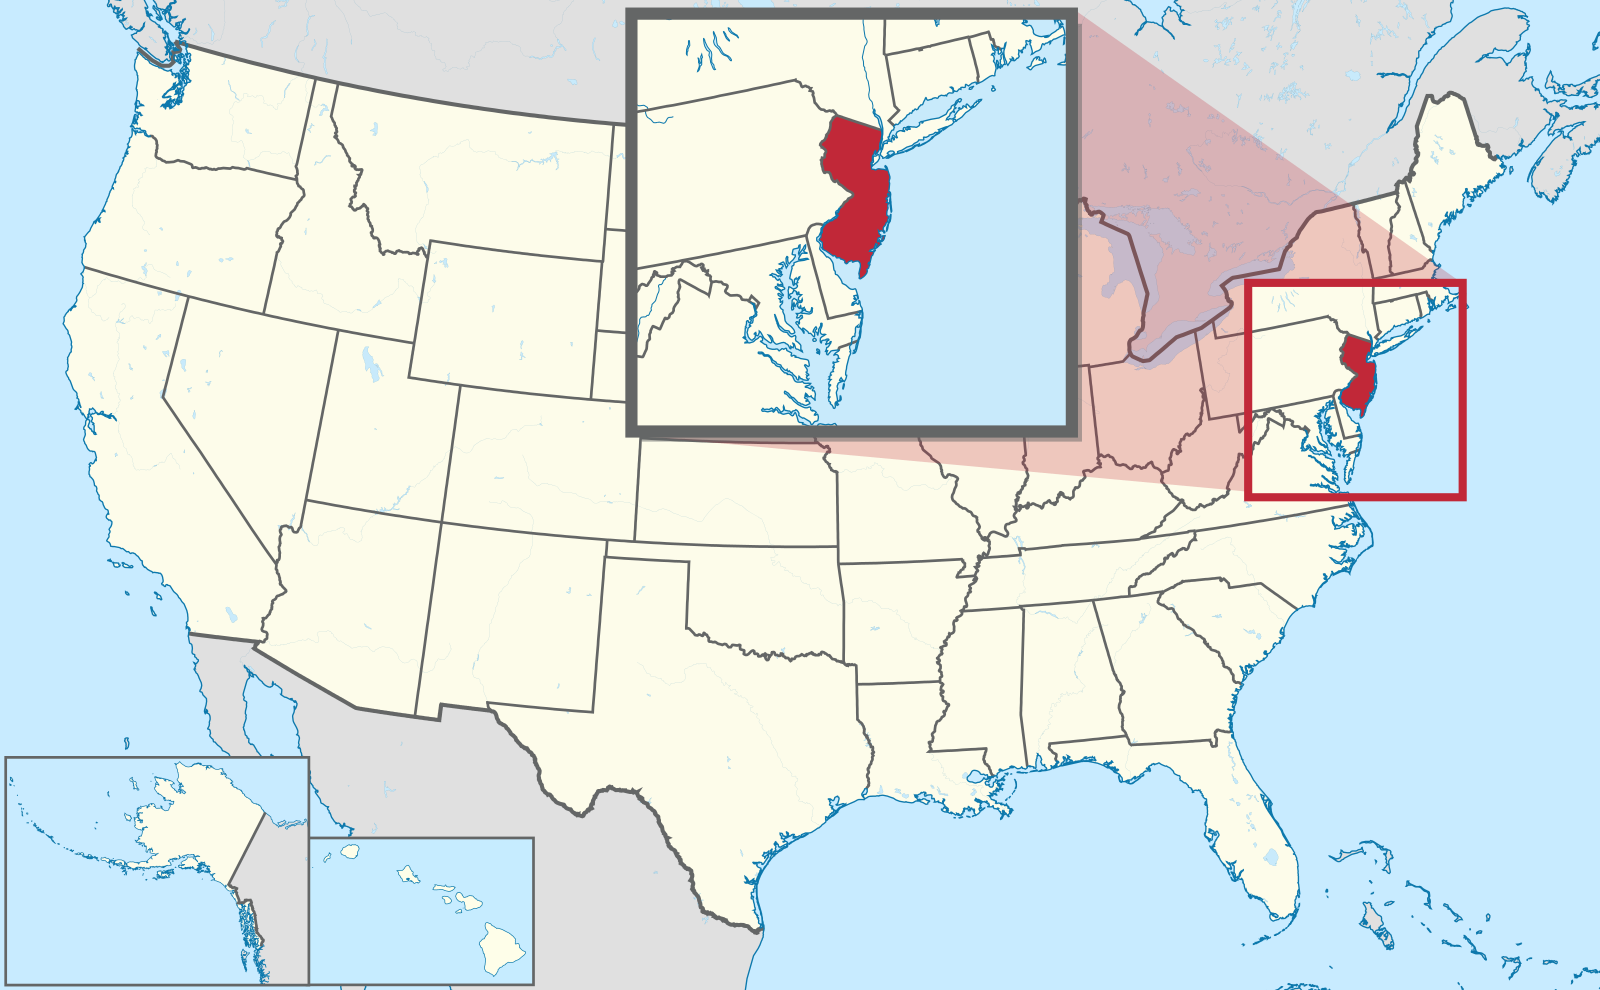
\includegraphics[width = \textwidth]{figures/nj_map}
\end{frame}

\begin{frame}
\begin{tikzpicture}[x = \textwidth, y = \textheight]
\node at (.5,.5) {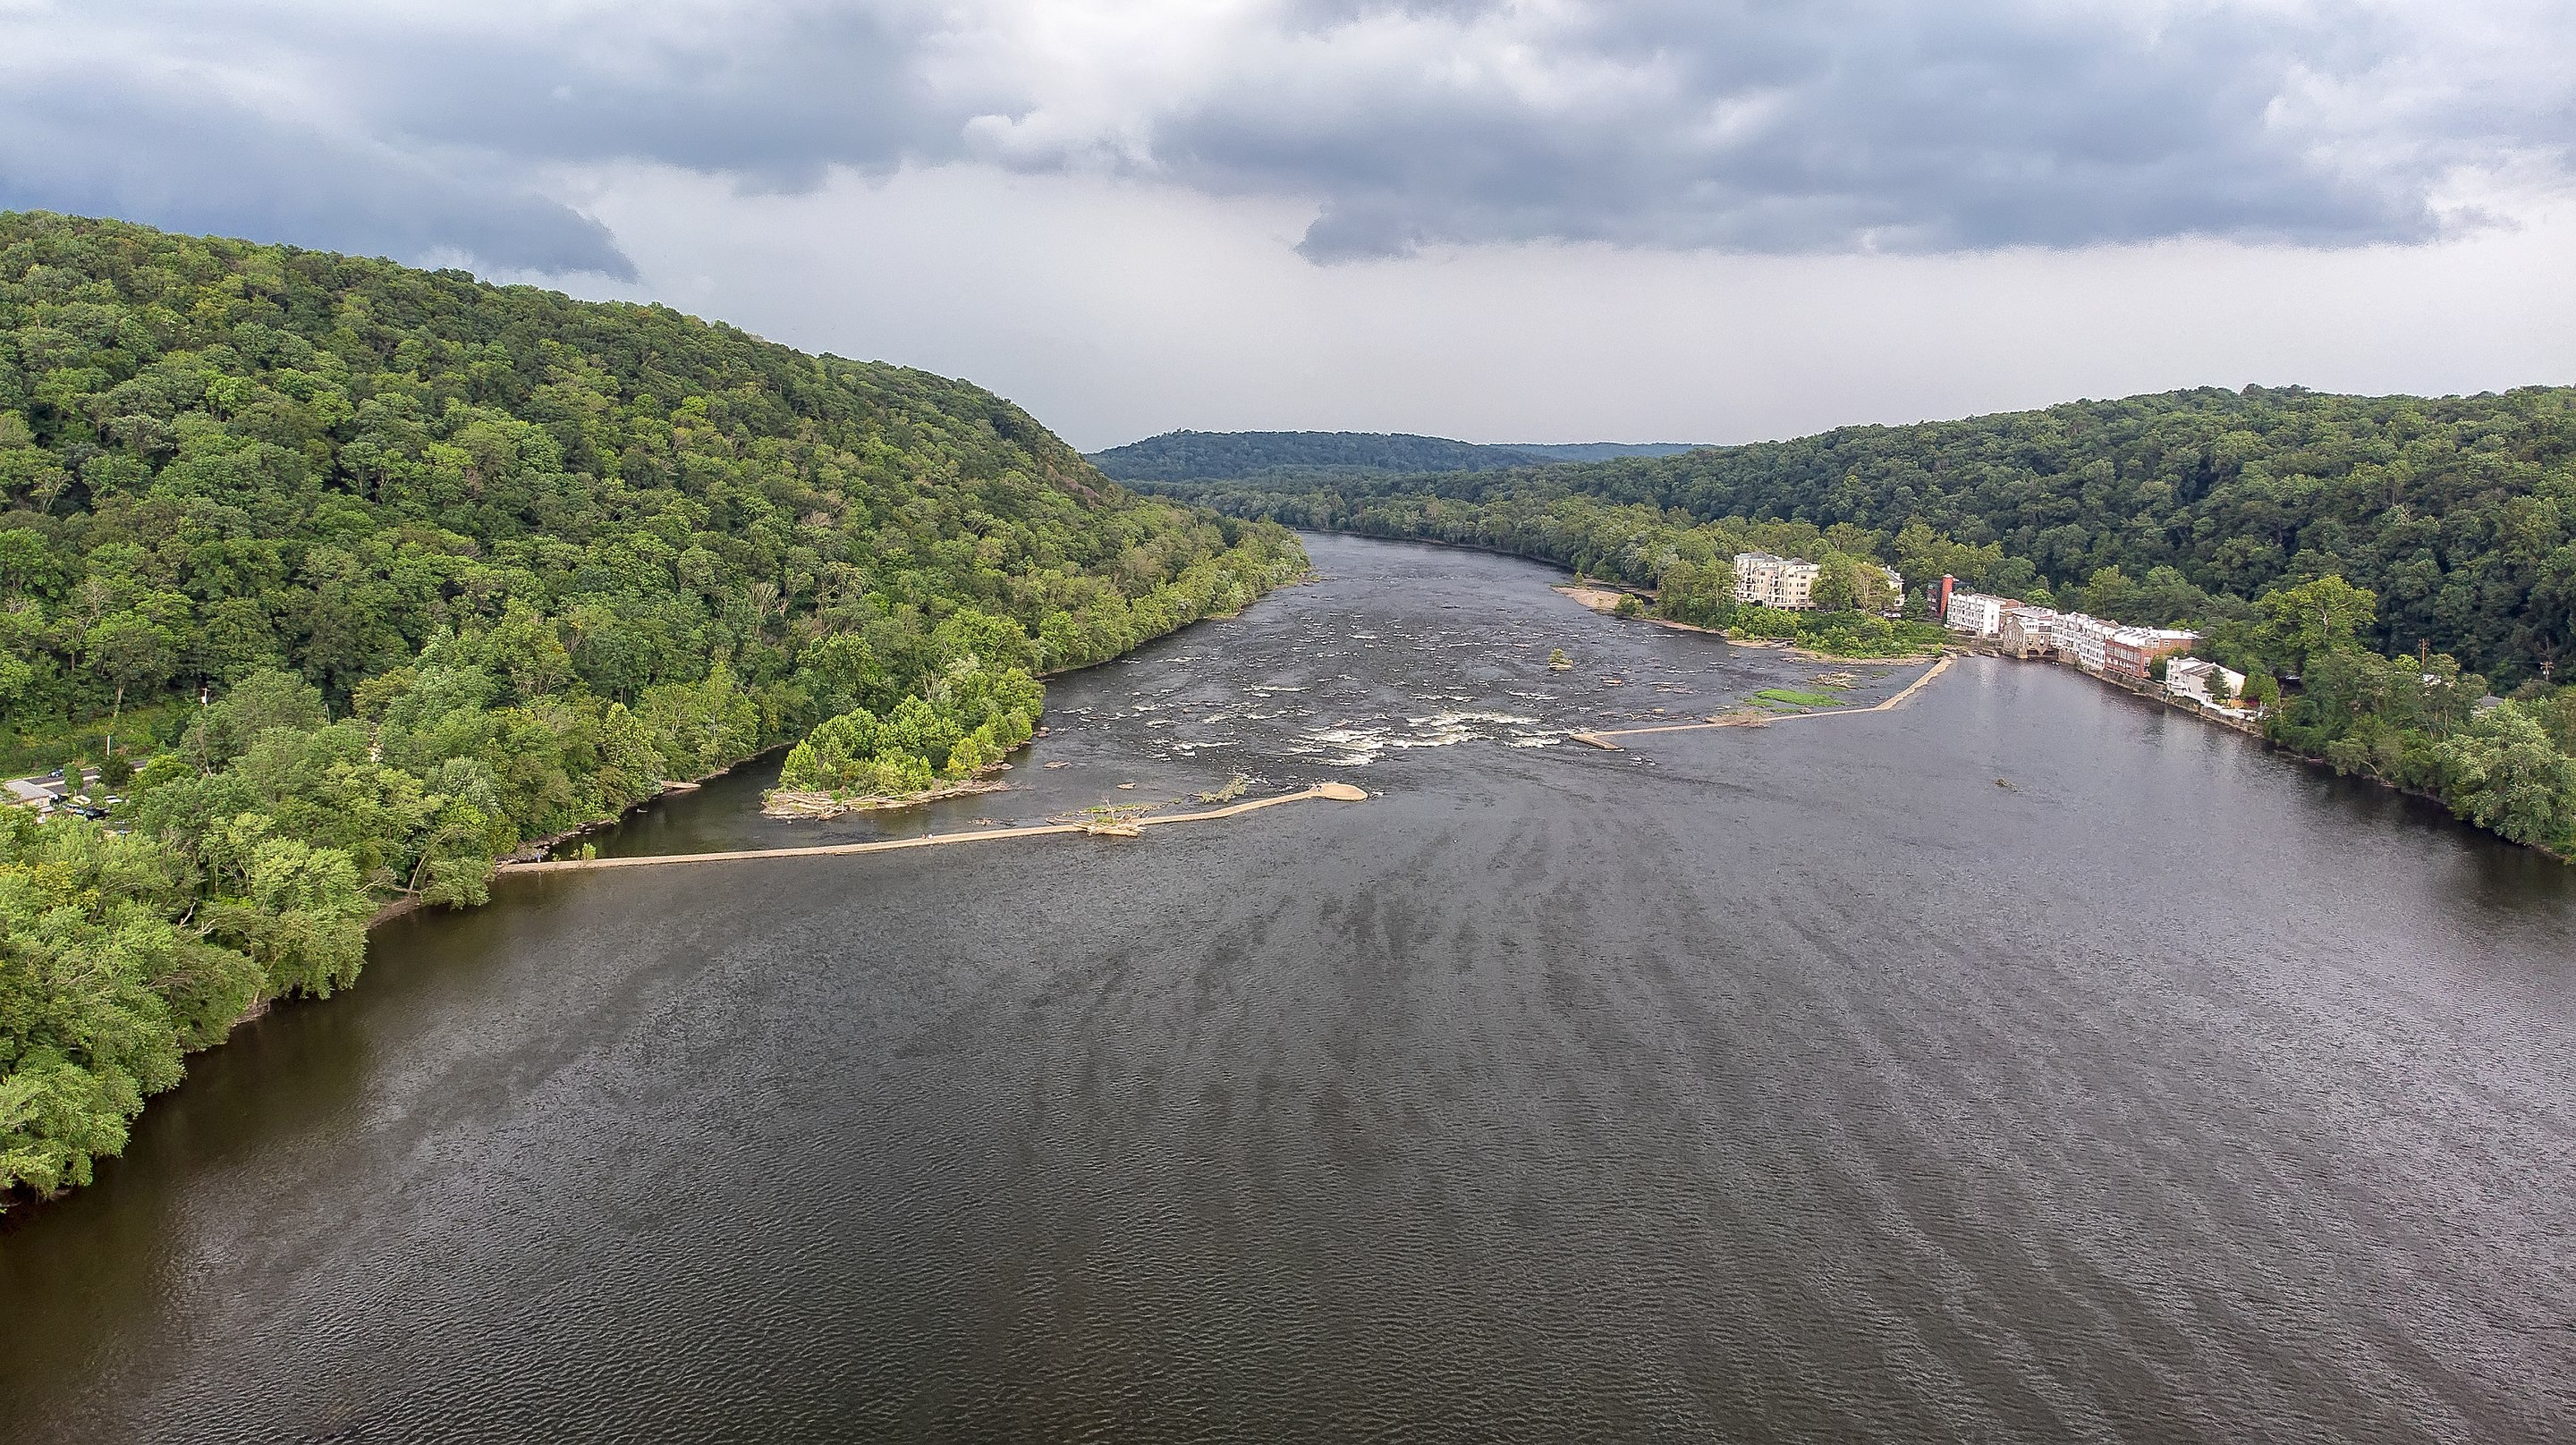
\includegraphics[width = \textwidth]{figures/Delaware_River}};
\node[anchor = south east, font = \tiny, align = center] at (1,0) {Photo by James Loesch - https://www.flickr.com/photos/jal33/49113053632/\\CC BY 2.0, https://commons.wikimedia.org/w/index.php?curid=87207834}; \pause
\node[anchor = north west, font = \bf, white, align = left] at (.03,.64) {New Jersey\\Minimum Wage\\Rose}; \pause
\node[anchor = north east, font = \bf, white, align = right] at (1,.64) {Pennsylvania\\No change};
\end{tikzpicture}
\end{frame}

\begin{frame}
\begin{tikzpicture}[x = \textwidth, y = \textheight]
\node at (0,0) {};
\node at (1,1) {};
\node[anchor = south] at (.2,.6) {
\includegraphics[width = .15\textwidth]{figures/burger_king}};
\node[anchor = south] at (.4,.6) {
\includegraphics[width = .15\textwidth]{figures/kfc}};
\node[anchor = south] at (.6,.6) {
\includegraphics[width = .15\textwidth]{figures/roy_rogers}};
\node[anchor = south] at (.8,.6) {
\includegraphics[width = .15\textwidth]{figures/wendys}};
\only<2->{
\node[anchor = north] at (.2,.6) {171 stores};
\node[anchor = north] at (.4,.6) {80 stores};
\node[anchor = north] at (.6,.6) {99 stores};
\node[anchor = north] at (.8,.6) {60 stores};
}
\only<3->{
\node[anchor = north west] at (0,.5) {Phone interview:};
\node[anchor = north west] at (.3,.5) {Feb-Mar 1992 before minimum wage rose};
\node[anchor = north west] at (.3,.44) {Nov-Dec 1992 after minimum wage rose};
}
\only<4->{
\node[anchor = north west] at (0, .35) {Recorded:};
\node[anchor = north west] at (.3, .35) {How many full-time equivalent employees?};
}
\end{tikzpicture}
\end{frame}

\begin{frame}
Did starting wages rise in NJ?
\end{frame}

\begin{frame}
\centering
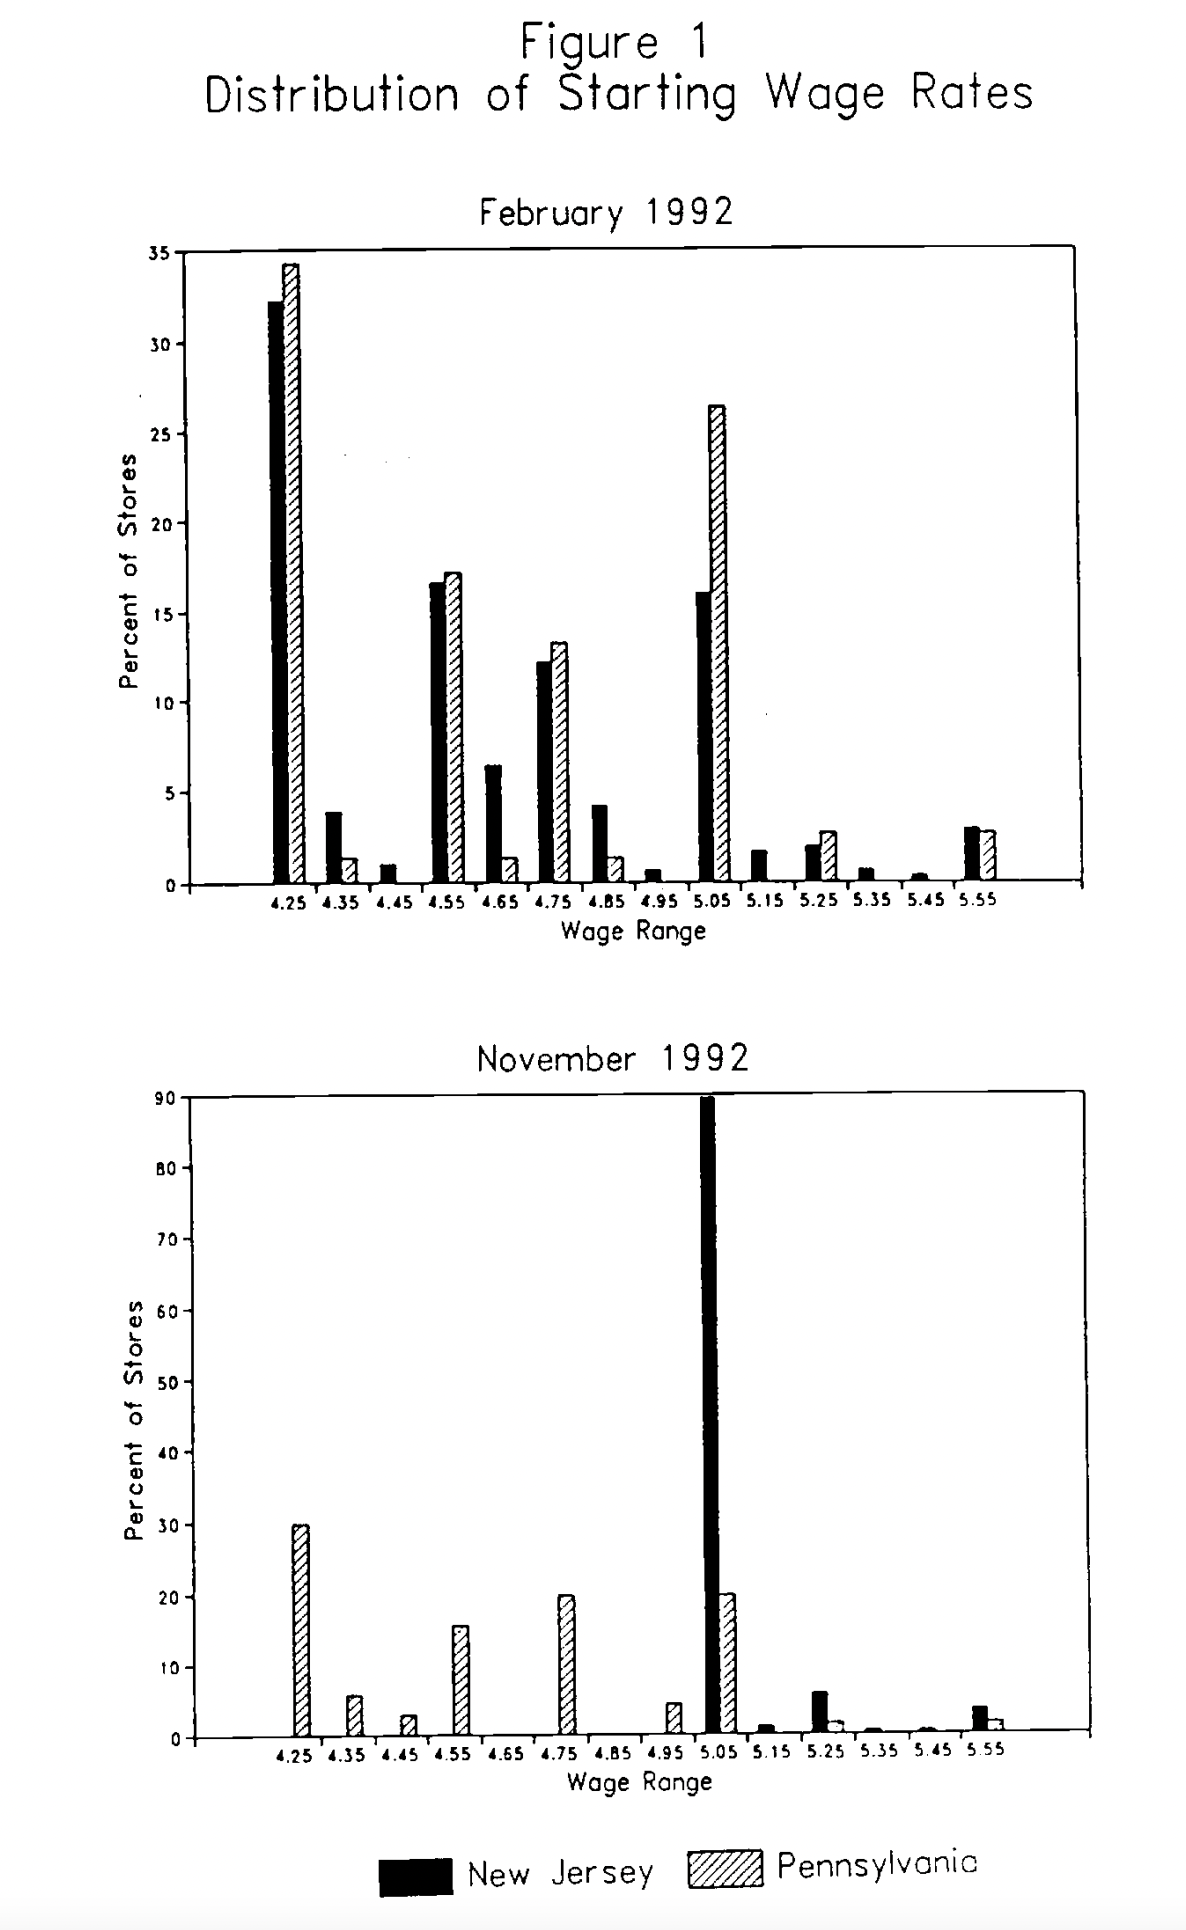
\includegraphics[height = \textheight]{figures/ck_fig1}
\end{frame}

\begin{frame}
How did employment change?
\end{frame}

\begin{frame}[t]

\includegraphics<1>[width = \textwidth]{figures/ck_slide1.pdf}
\includegraphics<2>[width = \textwidth]{figures/ck_slide2.pdf}
\includegraphics<3>[width = \textwidth]{figures/ck_slide3.pdf}
\includegraphics<4>[width = \textwidth]{figures/ck_slide4.pdf}
\includegraphics<5>[width = \textwidth]{figures/ck_slide5.pdf}

\end{frame}

\begin{frame}

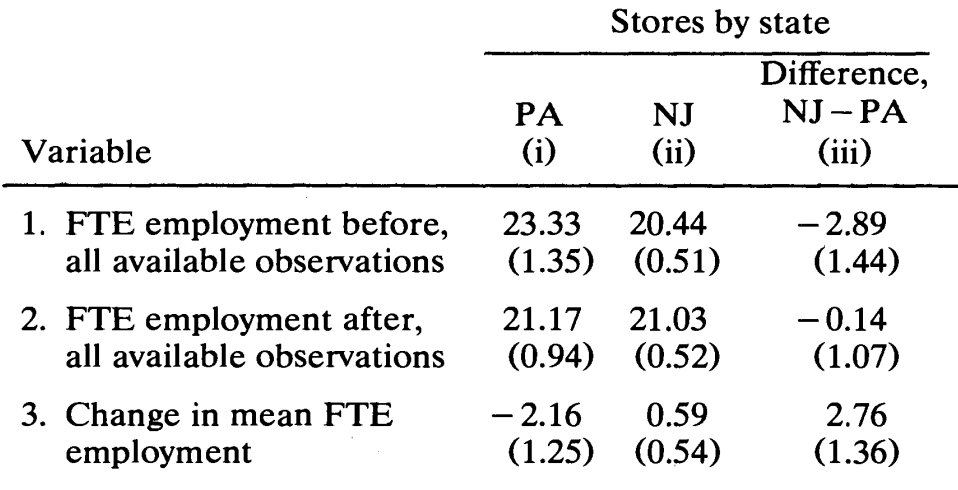
\includegraphics[width = .8\textwidth]{figures/ck_table}

\end{frame}

\begin{frame}

``Contrary to the central prediction of the textbook model of the minimum wage,...we find no evidence that the rise in New Jersey's minimum wage reduced employment at fast-food restaurants in the state.'' \vskip .5in

Card \& Krueger 1994, p.~792

\end{frame}

\begin{frame}

\begin{itemize}
\item simple study
\item well-executed
\item upended conventional wisdom
\end{itemize}

\end{frame}

\begin{frame}

\huge Key assumption: Parallel trends

\end{frame}

\begin{frame}
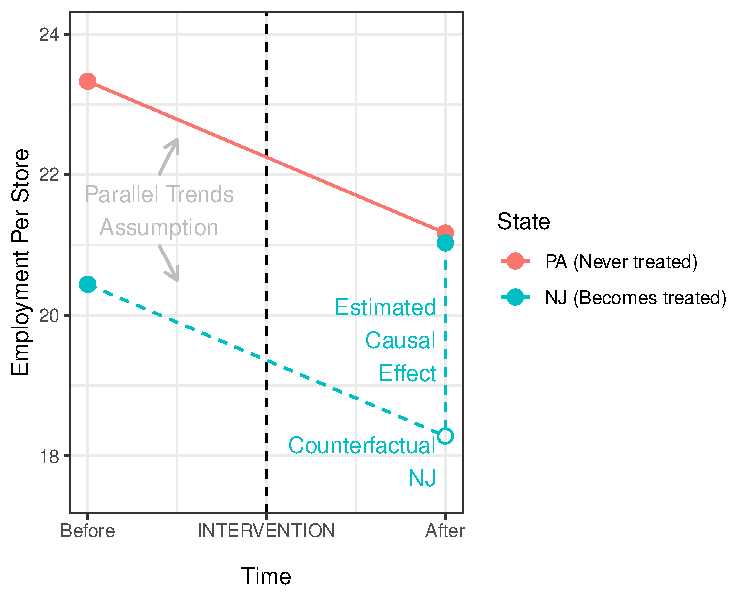
\includegraphics[width = .3\textwidth]{figures/ck_slide5.pdf} \vskip .1in \pause
\bgray{Parallel trends assumption:} \pause If no law had taken effect, then \pause
$$\overbrace{Y_\text{NJ,After}^0  - Y_\text{NJ,Before}^0}^\text{the trend in NJ} \overbrace{=}^\text{would equal} \overbrace{Y_\text{PA,After}^0 - Y_\text{PA,Before}^0}^\text{the trend in PA} $$ \pause
Rearranging yields a formula for the counterfactual outcome \pause
$$
\underbrace{Y_\text{NJ,After}^0}_\text{Counterfactual} \overbrace{=}^\text{By Assumption} \pause \underbrace{Y_\text{NJ,Before}^0 + Y_\text{PA,After}^0 - Y_\text{PA,Before}^0}_\text{Factual}
$$ \pause
$$\text{Effect in NJ} = \underbrace{Y_\text{NJ,After}^1}_\text{Observed}\quad  - \underbrace{Y_\text{NJ,After}^0}_\text{Estimated by Above}$$
\end{frame}

\begin{frame}{Can we test the parallel trends assumption?}

\onslide<2->{\bred{No.}}
\only<1>{$$\overbrace{Y_\text{NJ,After}^0  - Y_\text{NJ,Before}^0}^\text{Assumption: The trend in NJ} \overbrace{=}^\text{would equal} \overbrace{Y_\text{PA,After}^0 - Y_\text{PA,Before}^0}^\text{the trend in PA} $$}
\only<2->{$$\overbrace{\begin{red}\underbrace{Y_\text{NJ,After}^0}_\text{Not Observable}\end{red}  - Y_\text{NJ,Before}^0}^\text{Assumption: The trend in NJ} \overbrace{=}^\text{would equal} \overbrace{Y_\text{PA,After}^0 - Y_\text{PA,Before}^0}^\text{the trend in PA} $$} \vskip .2in
\onslide<3->{You can make it credible by looking at many pre-treatment periods}

\end{frame}

\begin{frame}[t]{DID would be very credible}
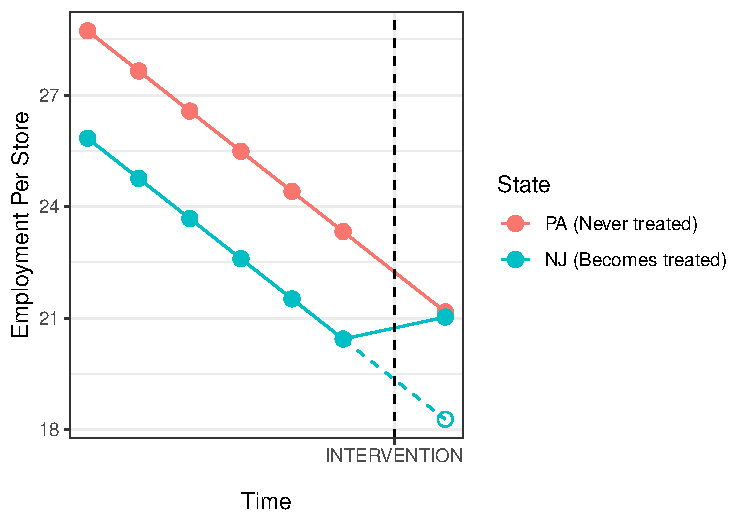
\includegraphics[width = \textwidth]{figures/parallel_trends_credible.pdf}
\end{frame}

\begin{frame}[t]{DID would be very doubtful}
\includegraphics<1>[width = \textwidth]{figures/parallel_trends_doubtful.pdf}
\includegraphics<2>[width = \textwidth]{figures/parallel_trends_doubtful_2.pdf}
\includegraphics<3>[width = \textwidth]{figures/parallel_trends_doubtful_3.pdf}
\end{frame}


\begin{frame}
Egami, N., \& Yamauchi, S. (2023).\\\bref{https://doi.org/10.1017/pan.2022.8}{Using multiple pretreatment periods to improve difference-in-differences and staggered adoption designs.}\\Political Analysis, 31(2), 195-212.
\end{frame}

\begin{frame}{Difference in difference}
\begin{tikzpicture}[x = \textwidth, y = .9\textheight]
\node at (0,0) {};
\node at (1,1) {};
\node[anchor = north west] (ey) at (0,1) {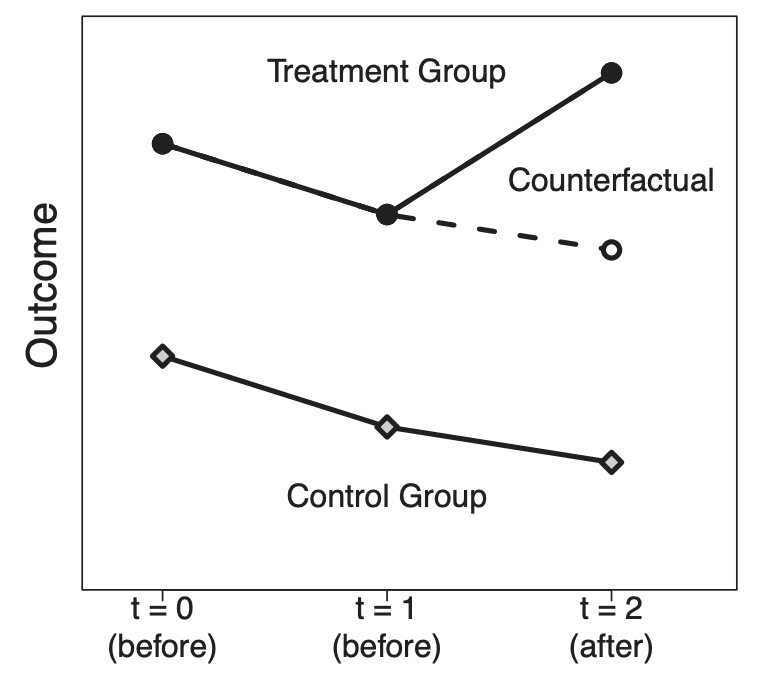
\includegraphics[width = .4\textwidth]{figures/egami_yamauchi_fig2a}}; 
\pause
\node[anchor = north, font = \large] (not) at (ey.south) {Notation};
\draw (not.south west) -- (not.south east);
\node[anchor = north, font = \large] (not2) at (not.south) {$Y_{\text{(unit)(time)}}^{\text{treatment value}}$};
\node[anchor = north, font = \large, align = left] (not3) at (not2.south) {Example: $Y_{i1}^0$\\is unit $i$ at time 1\\under treatment 0};
\pause
\node[anchor = north west, align = left] (pt) at (.5,1) {Parallel Trends Assumption\\(untestable)};
\draw[thick] (pt.south west) -- (pt.south east);
\node[anchor = north west, align = center] at (pt.south west) {$E(Y_{\text{Treated,2}}^0 - Y_{\text{Treated,1}}^0)$\\$=$\\$E(Y_{\text{Control,2}}^0 - Y_{\text{Control,1}}^0)$};
\pause
\node[anchor = north west, align = left] (ept) at (.5,.6) {Extended Parallel Trends\\(testable)};
\draw[thick] (ept.south west) -- (ept.south east);
\node[anchor = north west, align = center] at (ept.south west) {$E(Y_{\text{Treated,1}}^0 - Y_{\text{Treated,0}}^0)$\\$=$\\$E(Y_{\text{Control,1}}^0 - Y_{\text{Control,0}}^0)$};
\end{tikzpicture}

\begin{center}
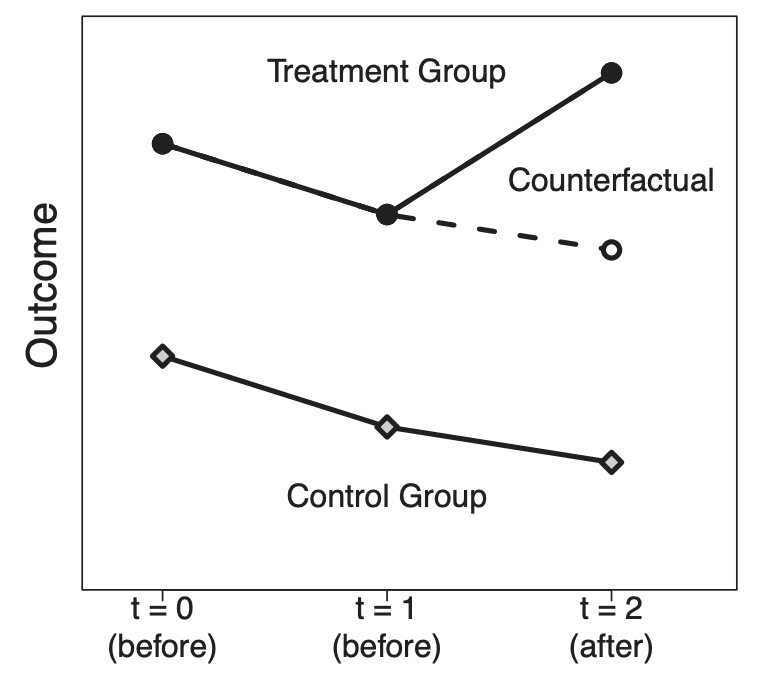
\includegraphics[width = .4\textwidth]{figures/egami_yamauchi_fig2a} \vskip .2in
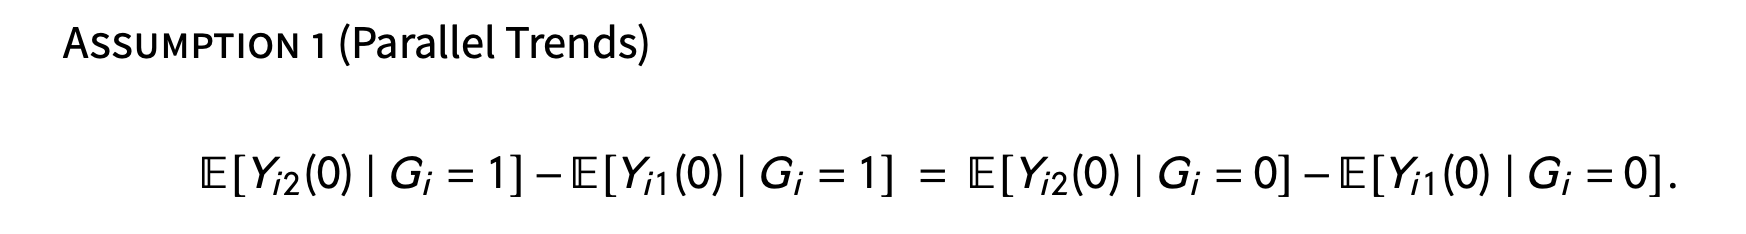
\includegraphics[width = \textwidth]{figures/ey_assumption_1}
\end{center}

\end{frame}

\begin{frame}
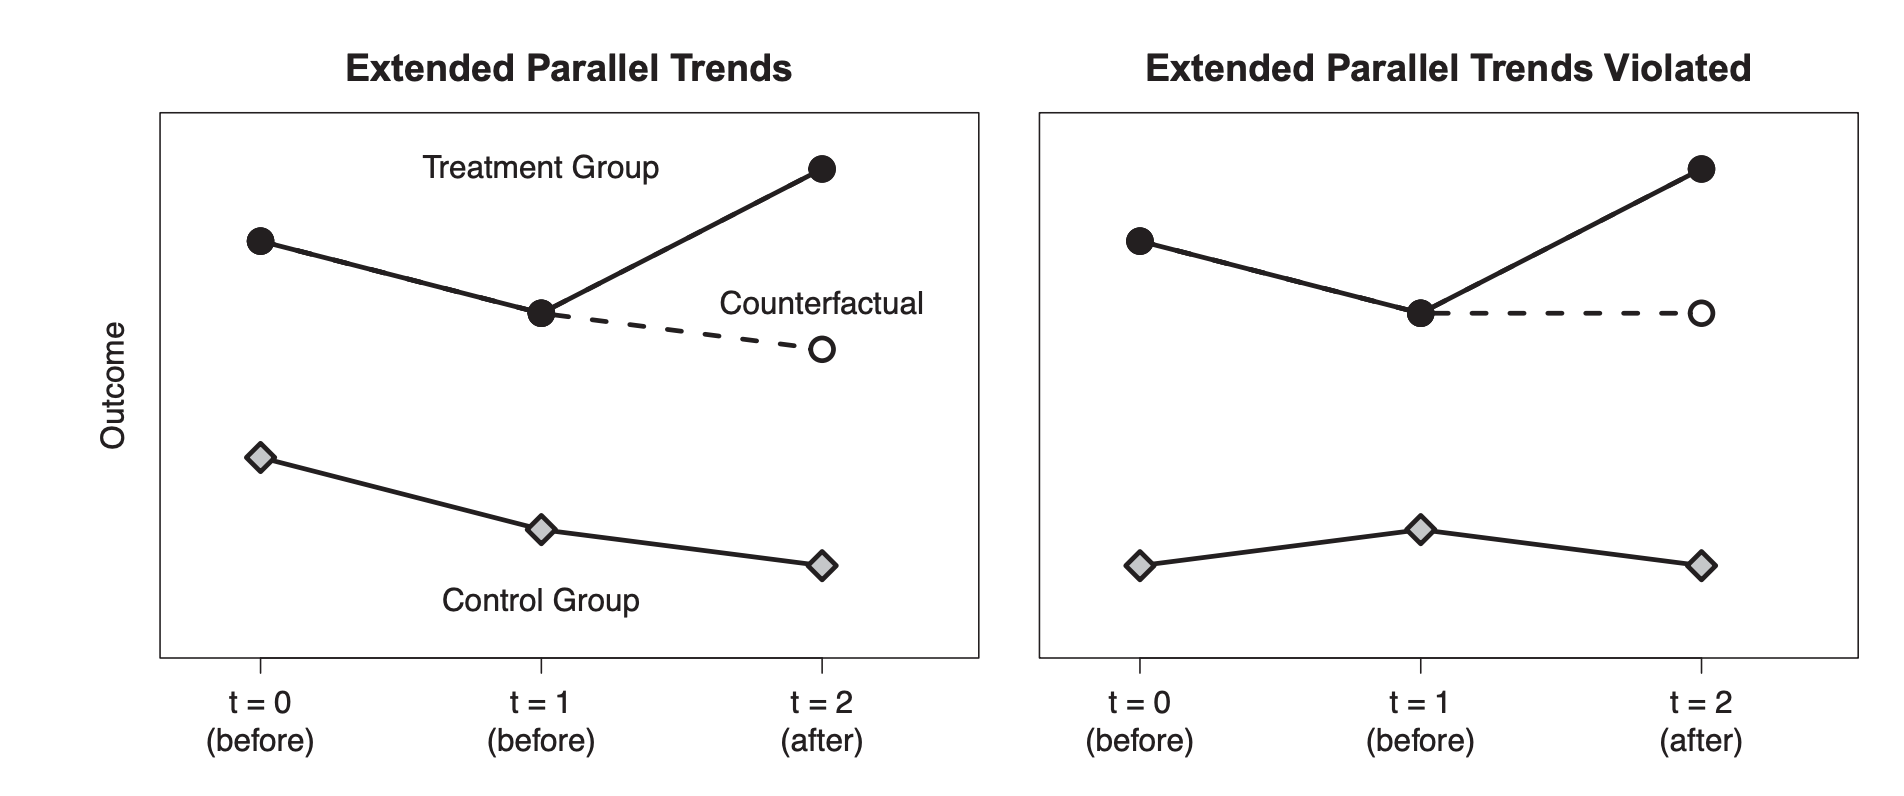
\includegraphics[width = \textwidth]{figures/ey_ept}
\end{frame}

\begin{frame}

Malesky, E. J., Nguyen, C. V., \& Tran, A. (2014).\\
\bref{https://doi.org/10.1017/S0003055413000580}{The impact of recentralization on public services:\\A difference-in-differences analysis of the abolition of elected councils in Vietnam.}\\
American Political Science Review, 108(1), 144-168.

\end{frame}

\begin{frame}

Does government work better when it is centralized or decentralized?

\end{frame}

\begin{frame}{Vietnam setting: A study of recentralization}


\begin{tikzpicture}[x = \textwidth, y = .8\textheight]
\node at (0,0) {};
\node at (1,1) {};
\node[draw, rounded corners] (national) at (.45,.8) {National Assembly};
\node[draw, rounded corners] (provincial) at (.45,.6) {Provincial People's Committee};
\node[draw, rounded corners] (district) at (.45,.4) {District People's Committee};
\node[draw, rounded corners] (commune) at (.45,.2) {Commune People's Committee};
\draw[->, thick] (national) -- (provincial);
\draw[->, thick] (provincial) -- (district);
\draw[->, thick] (district) -- (commune);
\node[font = \footnotesize, anchor = east] at (1,.8) {most centralized};
\node[font = \footnotesize, anchor = east] at (1,.4) {district $\approx$ 120k people};
\node[font = \footnotesize, anchor = east] at (1,.2) {most decentralized};
\draw[line width = 2pt, red] (district.west) -- (district.east);
\node[font = \footnotesize, anchor = west, red, align = left] at (0,.4) {National Assembly\\2008 Resolution\\to Study\\Removal of DPCs};
\end{tikzpicture}

\end{frame}

\begin{frame}{Vietnam setting: A study of recentralization}

Input from social scientists \pause
\begin{enumerate}
\item Enough treated units to study \pause
\item Sampling stratified by region \pause
\item Sampling stratified by
\begin{itemize}
\item city versus rural
\item lowland versus highland
\item midland versus inter-nationally bordered land
\end{itemize} \pause
\item Sampling stratified by socioeconomic and public administration performance
\end{enumerate}

\end{frame}

\begin{frame}
\centering
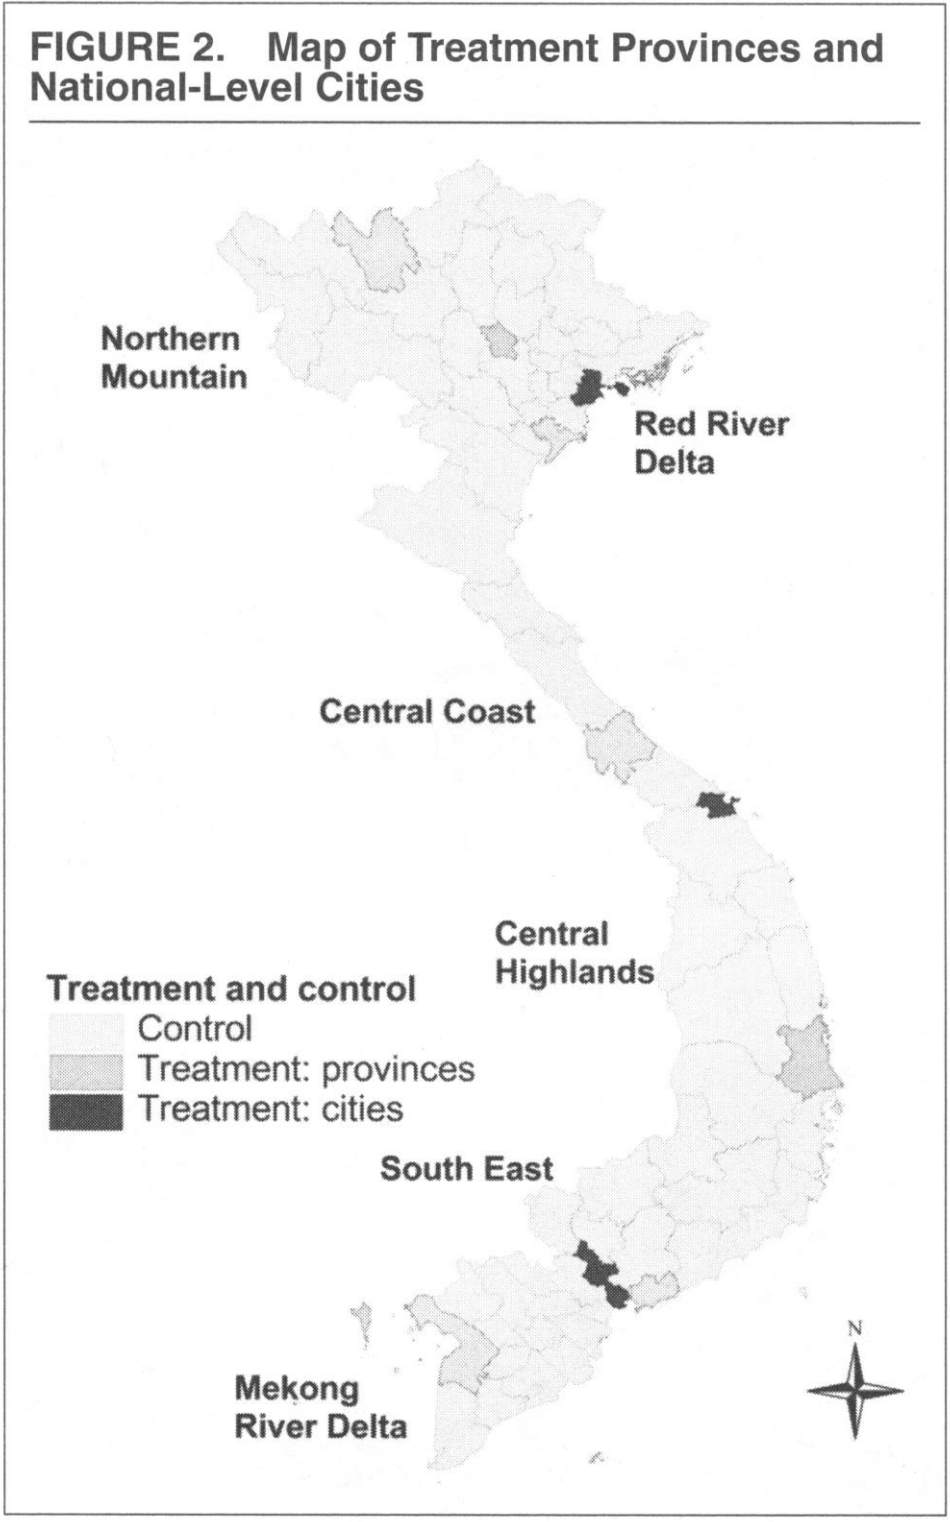
\includegraphics[height = .9\textheight]{figures/malesky_map}
\end{frame}

\begin{frame}

Vietnam Household Living Standards Survey\\
Reports by each local commune by commune leaders
\begin{itemize}
\item 2006 and 2008: Before DPC abolition
\item 2010: After DPC abolition
\end{itemize}
One outcome we will examine:\\
Is there the following project in the commune?
\begin{itemize}
\item Investment on culture and education
\end{itemize}

\end{frame}

\begin{frame}
\begin{tikzpicture}[x = \textwidth, y = .9\textheight]
\node at (0,0) {};
\node at (1,1) {};
\node[anchor = west] at (0,.5) {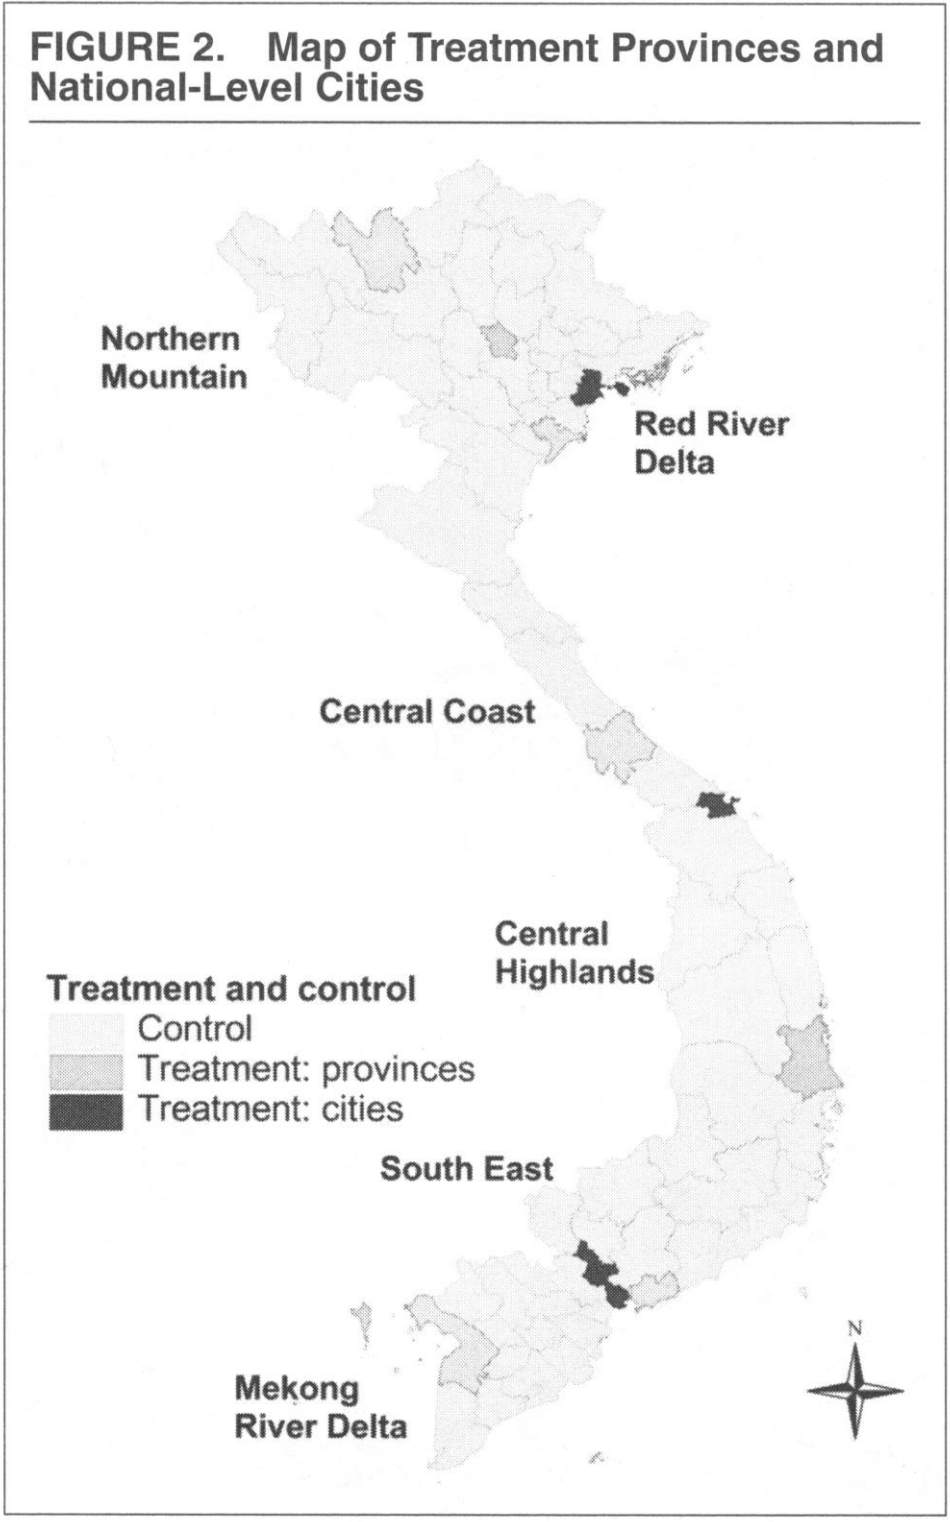
\includegraphics[height = .8\textheight]{figures/malesky_map}};
\onslide<2>{
\node[anchor = north west, align = left] at (.5,1) {Outcome 1\\Education and cultural programs};
\node[anchor = north west, align = left, font = \small, text width = .45\textwidth] at (.5,.85) {\raggedright Is there the following project in the commune?};
\node[anchor = north west, align = left, font = \small, text width = .45\textwidth] at (.55,.73) {\raggedright Investment on culture\\and education};
}
\onslide<3>{
\node[anchor = north west, align = left] at (.5,1) {Outcome 2\\Tap water};
\node[anchor = north west, align = left, font = \small, text width = .45\textwidth] at (.5,.85) {\raggedright Is there the following project in the commune?};
\node[anchor = north west, align = left, font = \small, text width = .45\textwidth] at (.55,.75) {\raggedright \bgray{Coded 1}\\Indoor private piped water\\
Outdoor private piped water\\
Public piped water};
\node[anchor = north west, align = left, font = \small, text width = .45\textwidth] at (.55,.53) {\raggedright \bgray{Coded 0}\\
Well water \\
Well with protection walls \\
Well without protection walls \\
Stream water with protection \\
Stream water without protection \\
Rainwater \\
Bottled water \\
Water brought by pedicab \\
Tank water \\
river lake pond};
}
\onslide<4>{
\node[anchor = north west, align = left] at (.5,1) {Outcome 3\\Agricultural center};
\node[anchor = north west, align = left, font = \small, text width = .45\textwidth] at (.5,.85) {\raggedright Is there any agriculture \\extension center\\in this commune?};
}
\end{tikzpicture}
\end{frame}

\begin{frame}
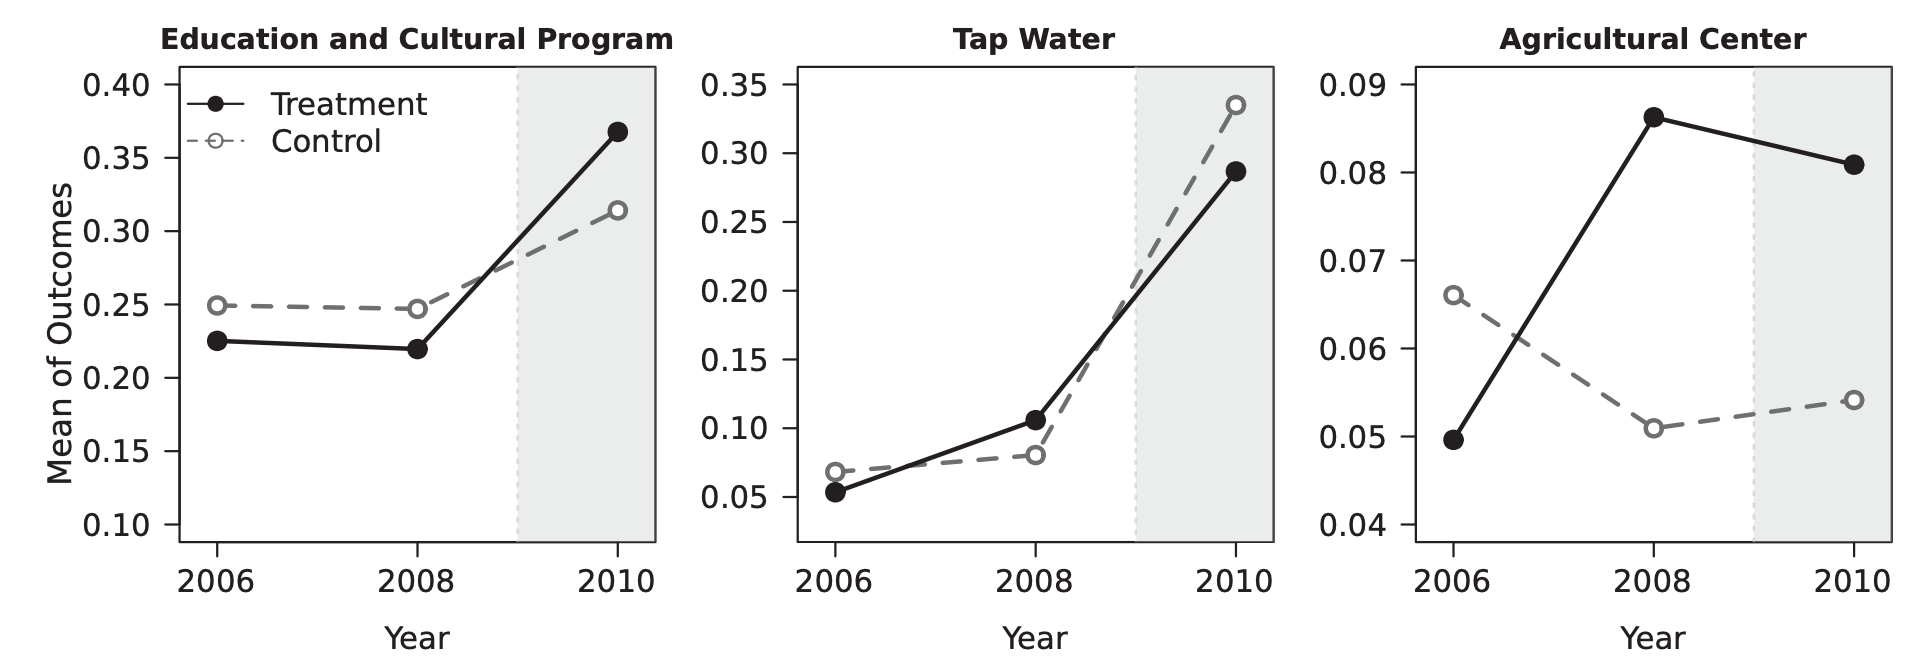
\includegraphics[width = \textwidth]{figures/ey_fig3} \pause \vskip .2in
In each case, do you believe parallel trends? \pause \vskip .2in
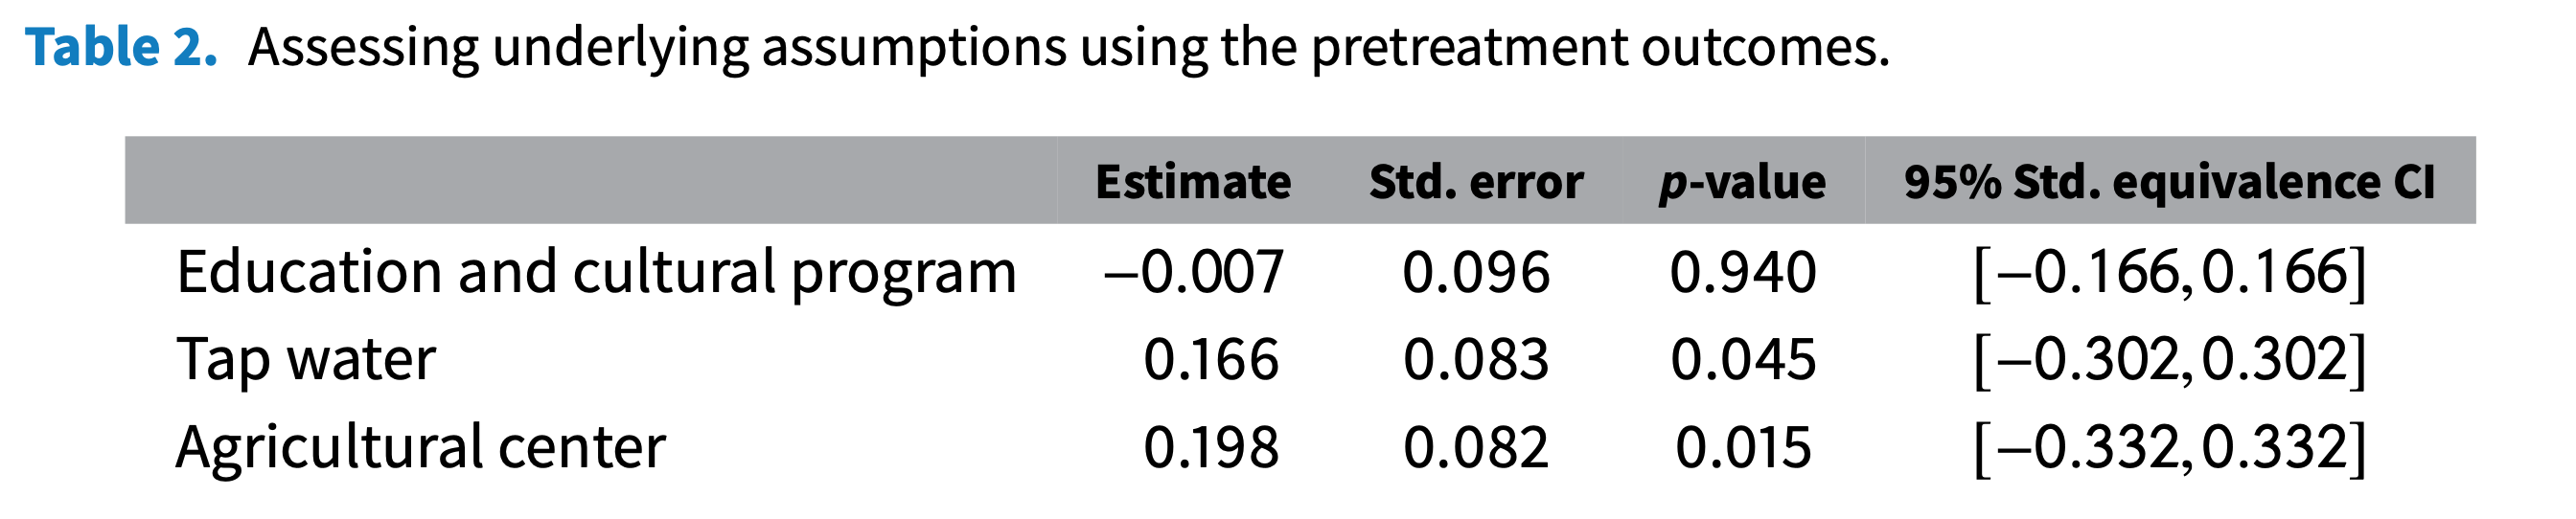
\includegraphics[width = \textwidth]{figures/ey_table2}
\end{frame}

\begin{frame}{Benefit 1: Assessing assumptions}

Pre-treatment periods enable us to\\\bblue{assess underlying ssumptions}\vskip .2in
Parallel trends is untestable, but being parallel \\
in the pre-treatment period builds confidence

\end{frame}

\begin{frame}{Benefit 2: Improving efficiency}

Pre-treatment periods also enable us to\\\bblue{improve estimation accuracy}\\when parallel trends holds

\end{frame}

\begin{frame}{Benefit 2: Improving efficiency}
\begin{tikzpicture}[x = \textwidth, y = .9\textheight]
\node at (0,0) {};
\node at (1,1) {};
\node[anchor = north west] (ey) at (0,1) {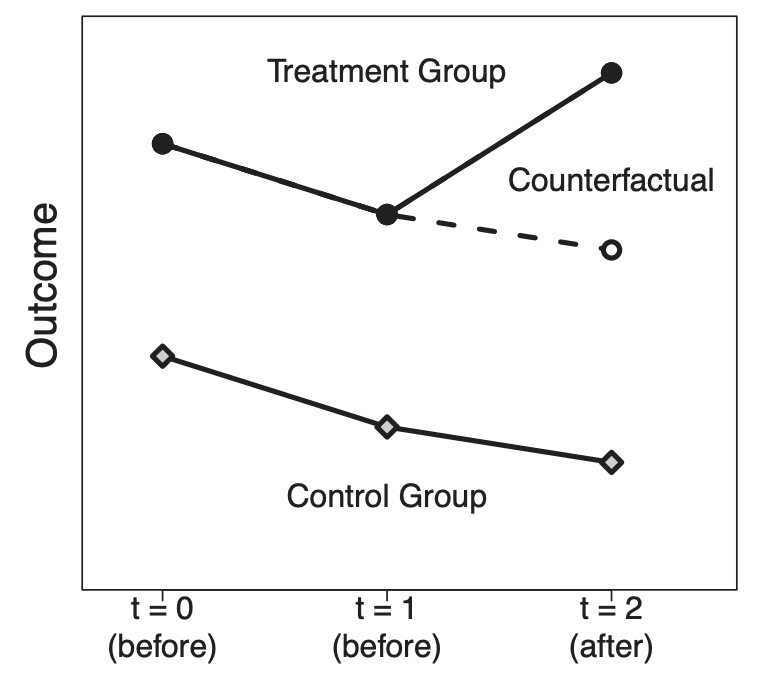
\includegraphics[width = .4\textwidth]{figures/egami_yamauchi_fig2a}}; 
\node[anchor = north, font = \large] (not) at (.25,.4) {Notation};
\draw (not.south west) -- (not.south east);
\node[anchor = north, font = \large] (not2) at (not.south) {$Y_{\text{(unit)(time)}}^{\text{treatment value}}$};
\node[anchor = north west] (est1) at (.5,1) {Estimator 1};
\node[anchor = north west] (est2) at (.5,.7) {Estimator 2};
\pause
\node[anchor = north west, align = center] at (est1.south west) {$\underbrace{(\bar{Y}_{T2}^1 - \bar{Y}_{T1}^0)}_{\substack{\text{Treatment Group}\\\text{Time 2 - Time 1}}}-\underbrace{(\bar{Y}_{C2}^0 - \bar{Y}_{C1}^0)}_{\substack{\text{Control Group}\\\text{Time 2 - Time 1}}}$};
\pause
\node[anchor = north west, align = center] at (est2.south west) {$\underbrace{(\bar{Y}_{T2}^1 - \bar{Y}_{T0}^0)}_{\substack{\text{Treatment Group}\\\text{Time 2 - Time 0}}}-\underbrace{(\bar{Y}_{C2}^0 - \bar{Y}_{C0}^0)}_{\substack{\text{Control Group}\\\text{Time 2 - Time 0}}}$};
\pause
\node[anchor = north west, font = \bf, blue, align = left] at (.5,.35) {Pooled estimator:\\Average the two!};
\end{tikzpicture}

\end{frame}

\begin{frame}{Benefit 2: Improving efficiency}
\centering
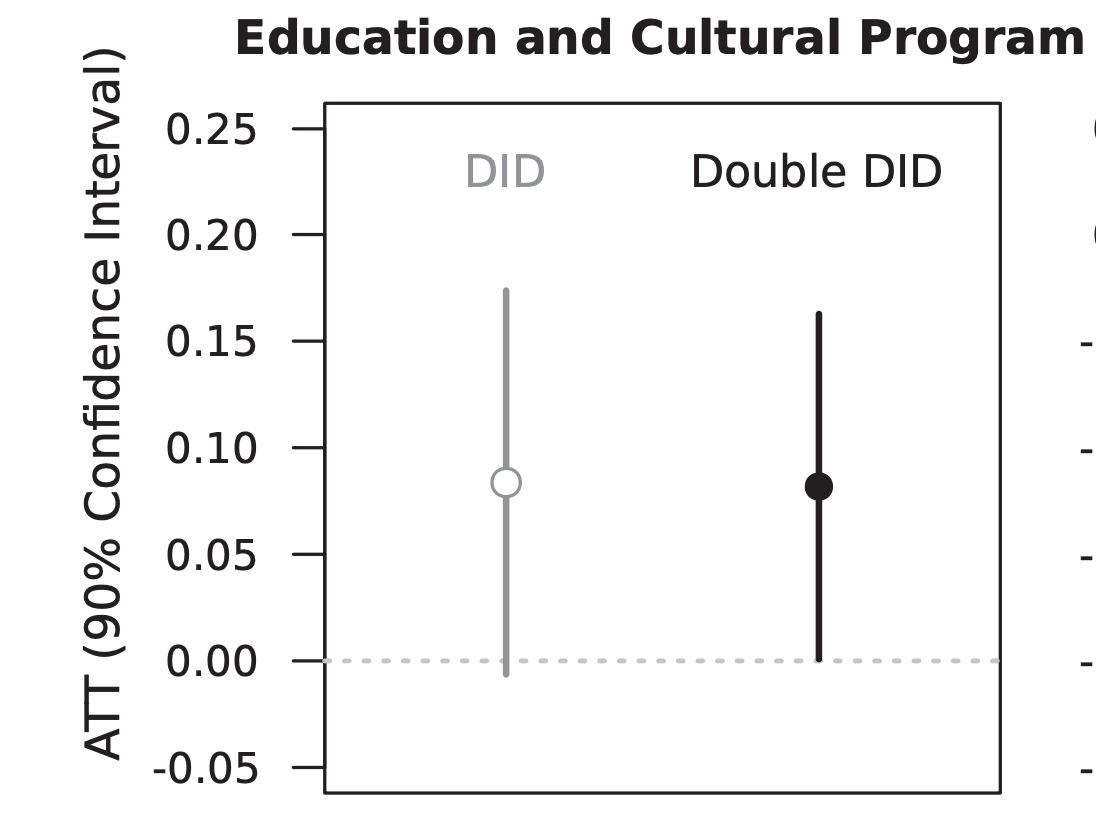
\includegraphics[width = .5\textwidth]{figures/ey_fig4a}
\end{frame}

\begin{frame}{Benefit 3: A more flexible assumption}

Pre-treatment periods make it possible to\\
\bblue{allow for a more flexible parallel trends assumption}

\end{frame}

\begin{frame}{Benefit 3: A more flexible assumption}
\begin{tikzpicture}[x = \textwidth, y = .9\textheight]
\node at (0,0) {};
\node at (1,1) {};
\node[anchor = west] at (0,.5) {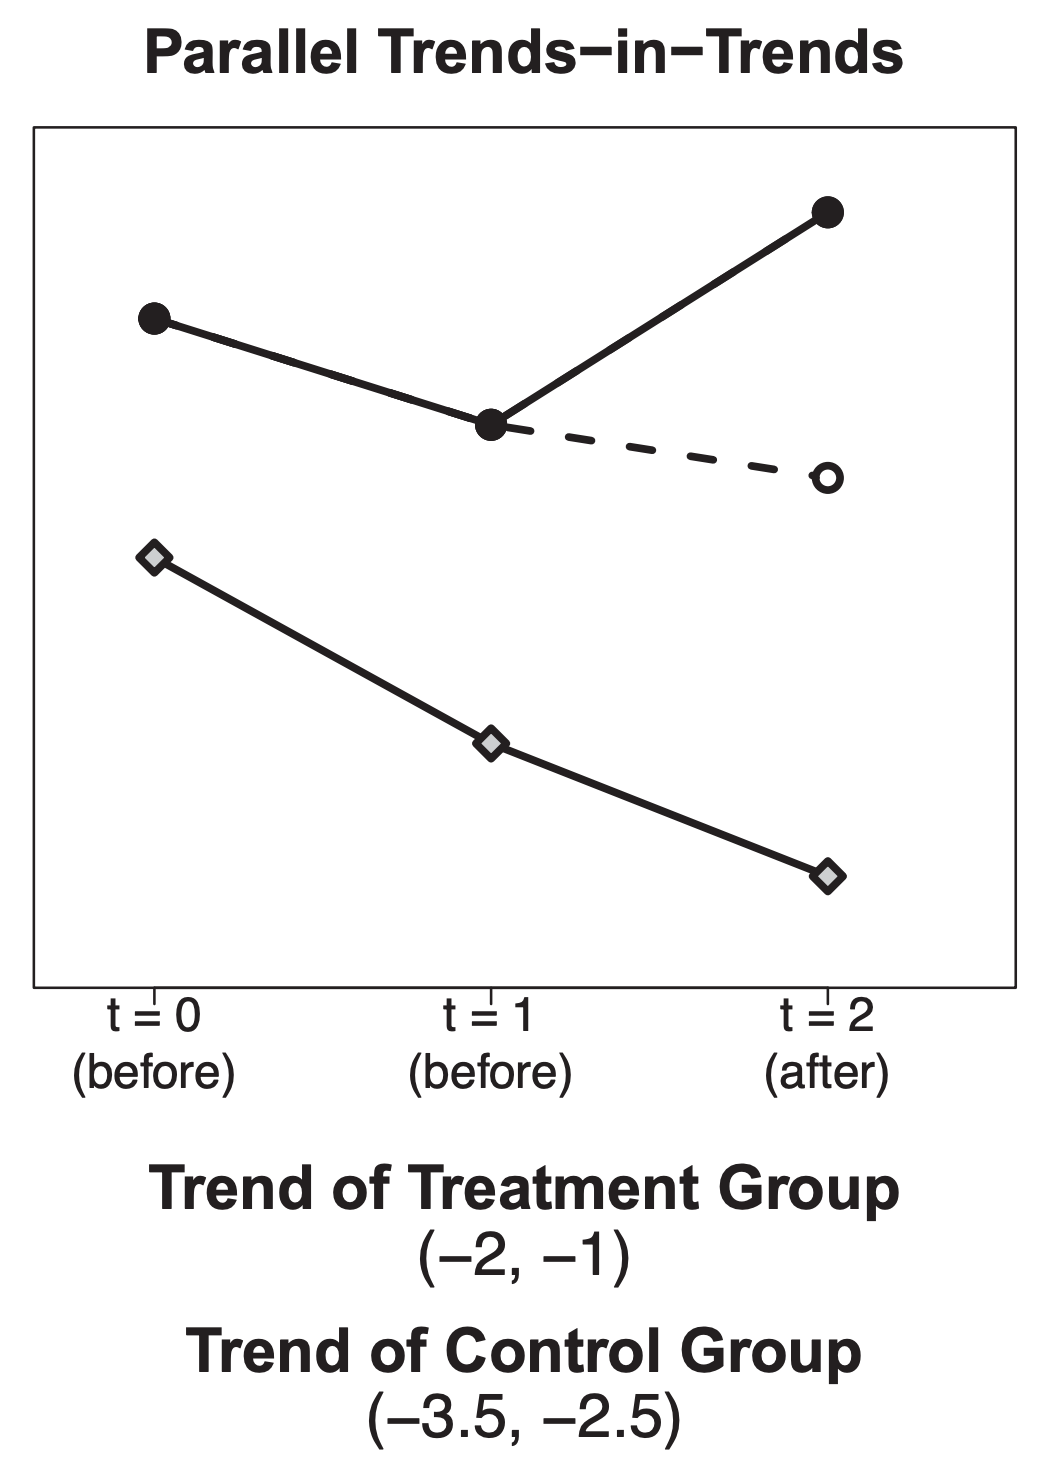
\includegraphics[height = .5\textheight]{figures/ey_fig2b}}; \pause
\node[anchor = north east] at (1,.8) {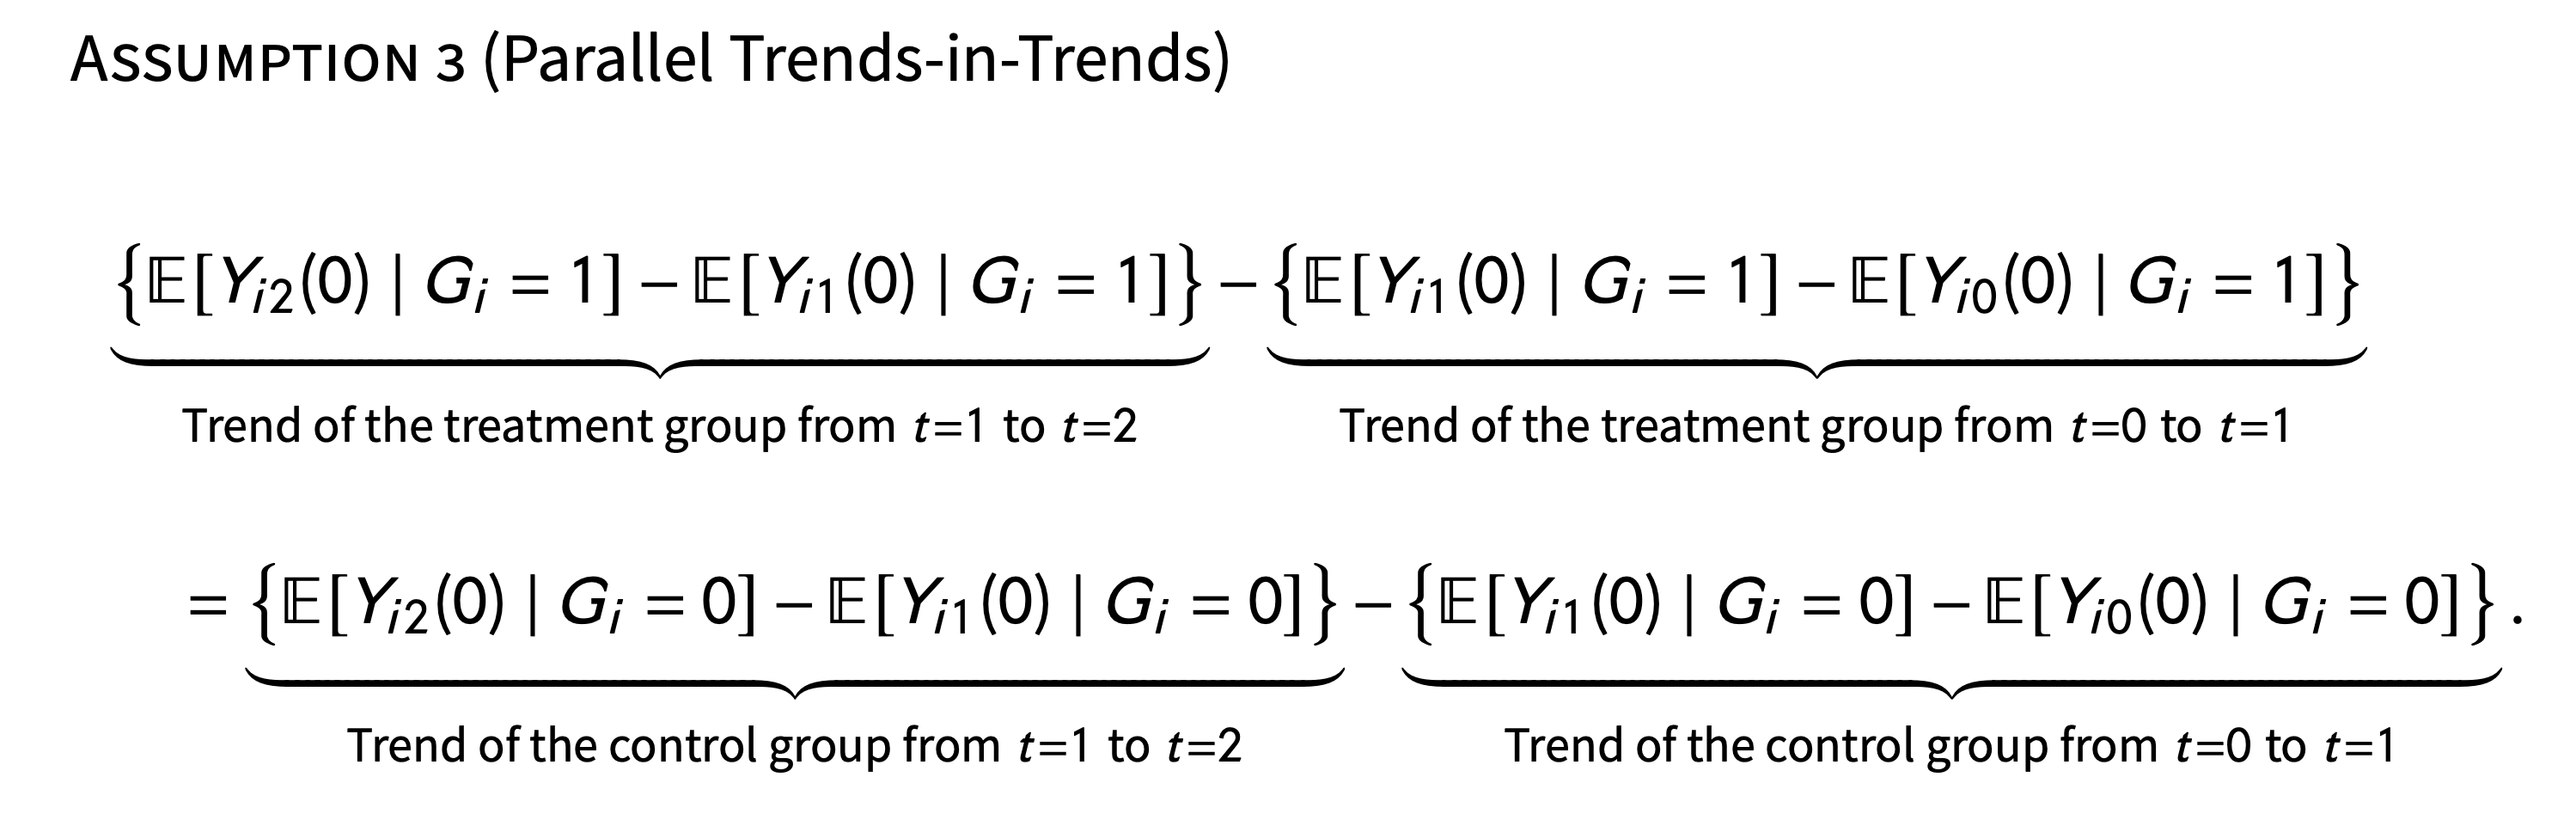
\includegraphics[width = .65\textwidth]{figures/ey_assumption3}}; \pause
\node[anchor = north west] at (.35,.47) {Sequential DID Estimator};
\node[anchor = north west] at (.35,.4) {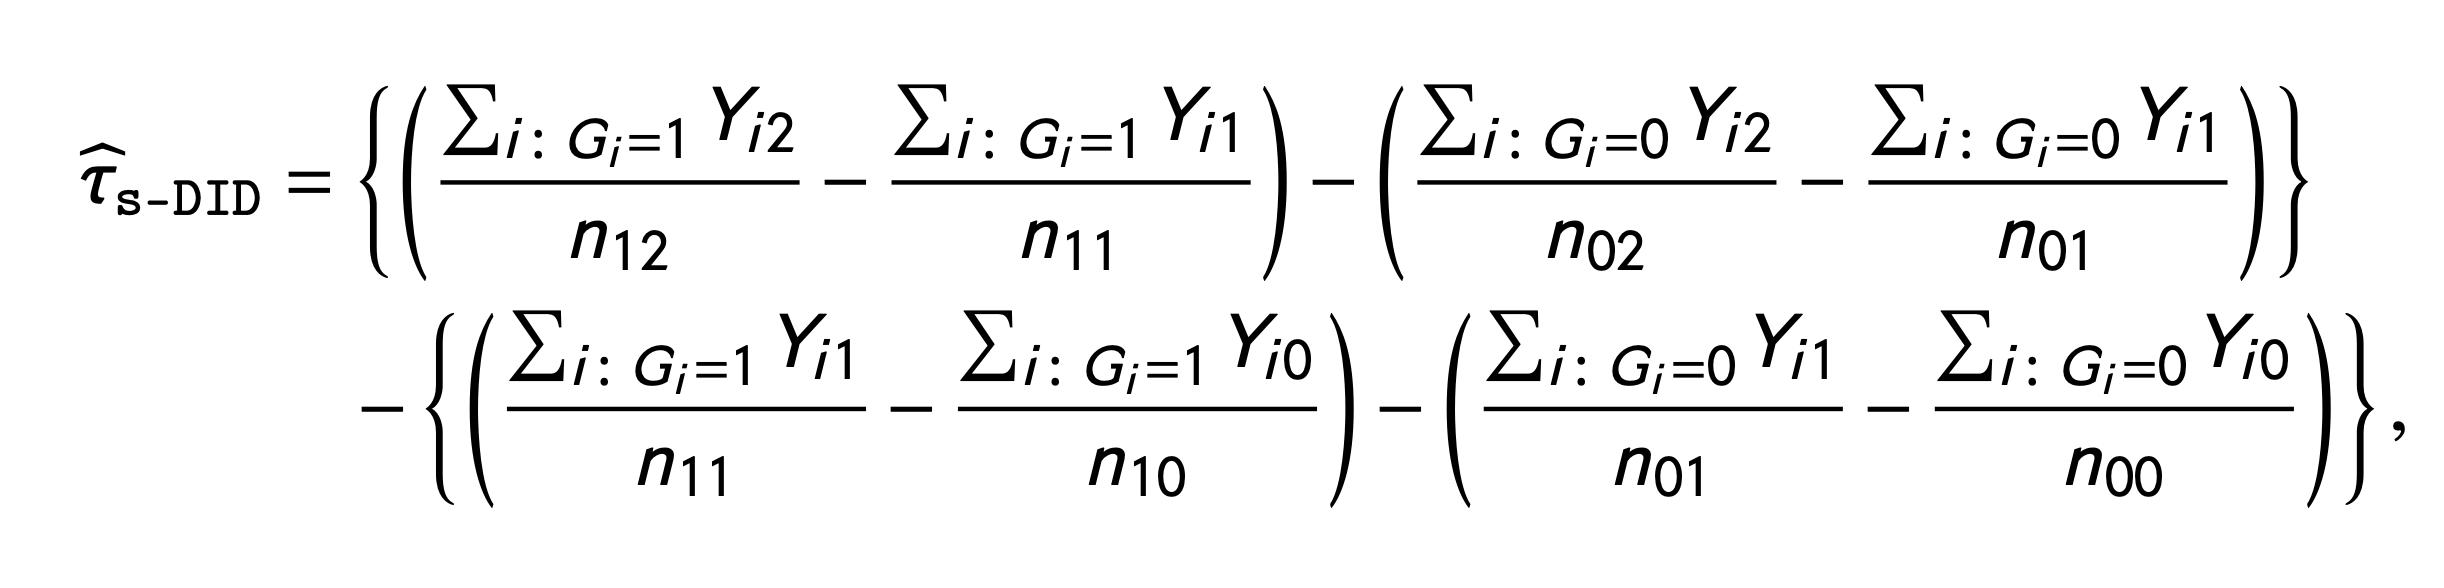
\includegraphics[width = .65\textwidth]{figures/ey_sdid}};
\end{tikzpicture}
\end{frame}

\begin{frame}{Benefit 3: A more flexible assumption}
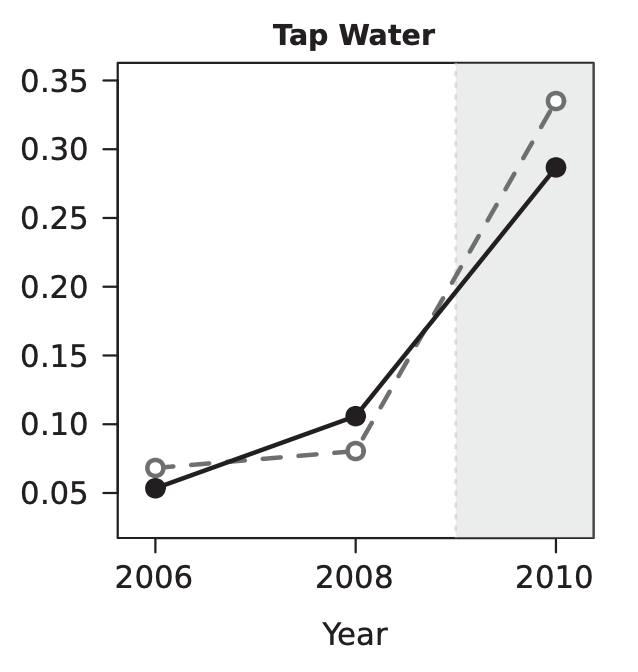
\includegraphics[width = .4\textwidth]{figures/ey_fig3b} \qquad
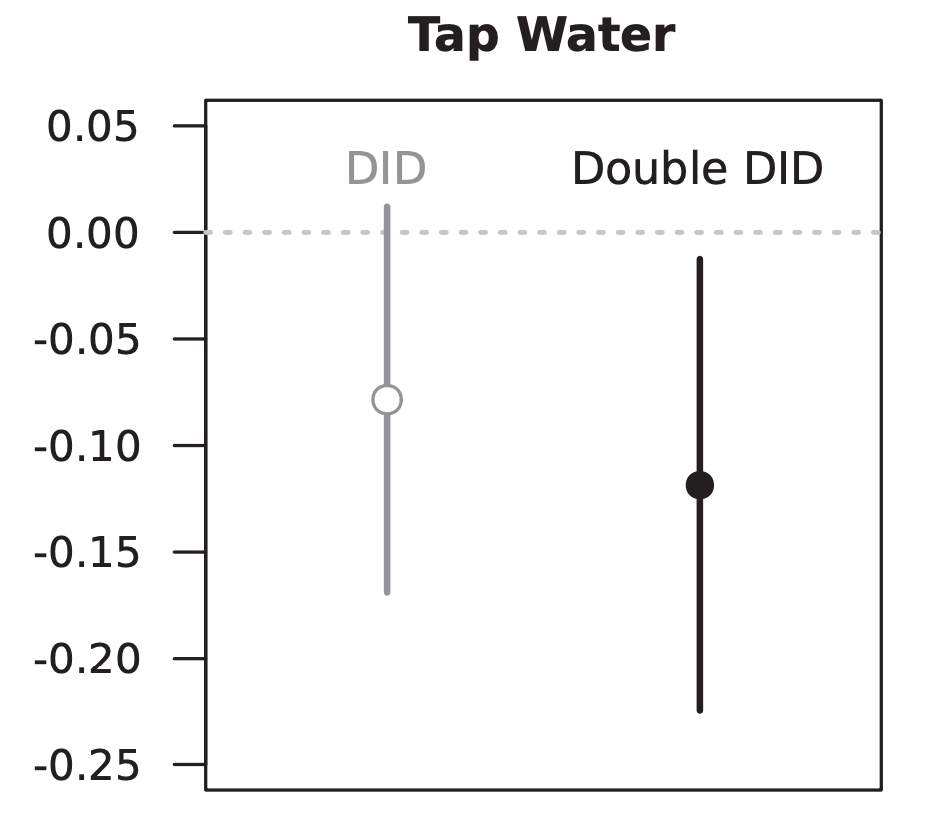
\includegraphics[width = .4\textwidth]{figures/ey_fig4b}
\end{frame}

\begin{frame}{Benefits of multiple pre-treatment periods}

\begin{enumerate}
\item assess underlying assumptions
\item improve estimation accuracy
\item allow for a more flexible parallel trends assumption
\end{enumerate}
\begin{tikzpicture}[x = \textwidth, y = .6\textheight]
\node at (0,0) {};
\node at (1,1) {};
\node<2> at (.5,.5) {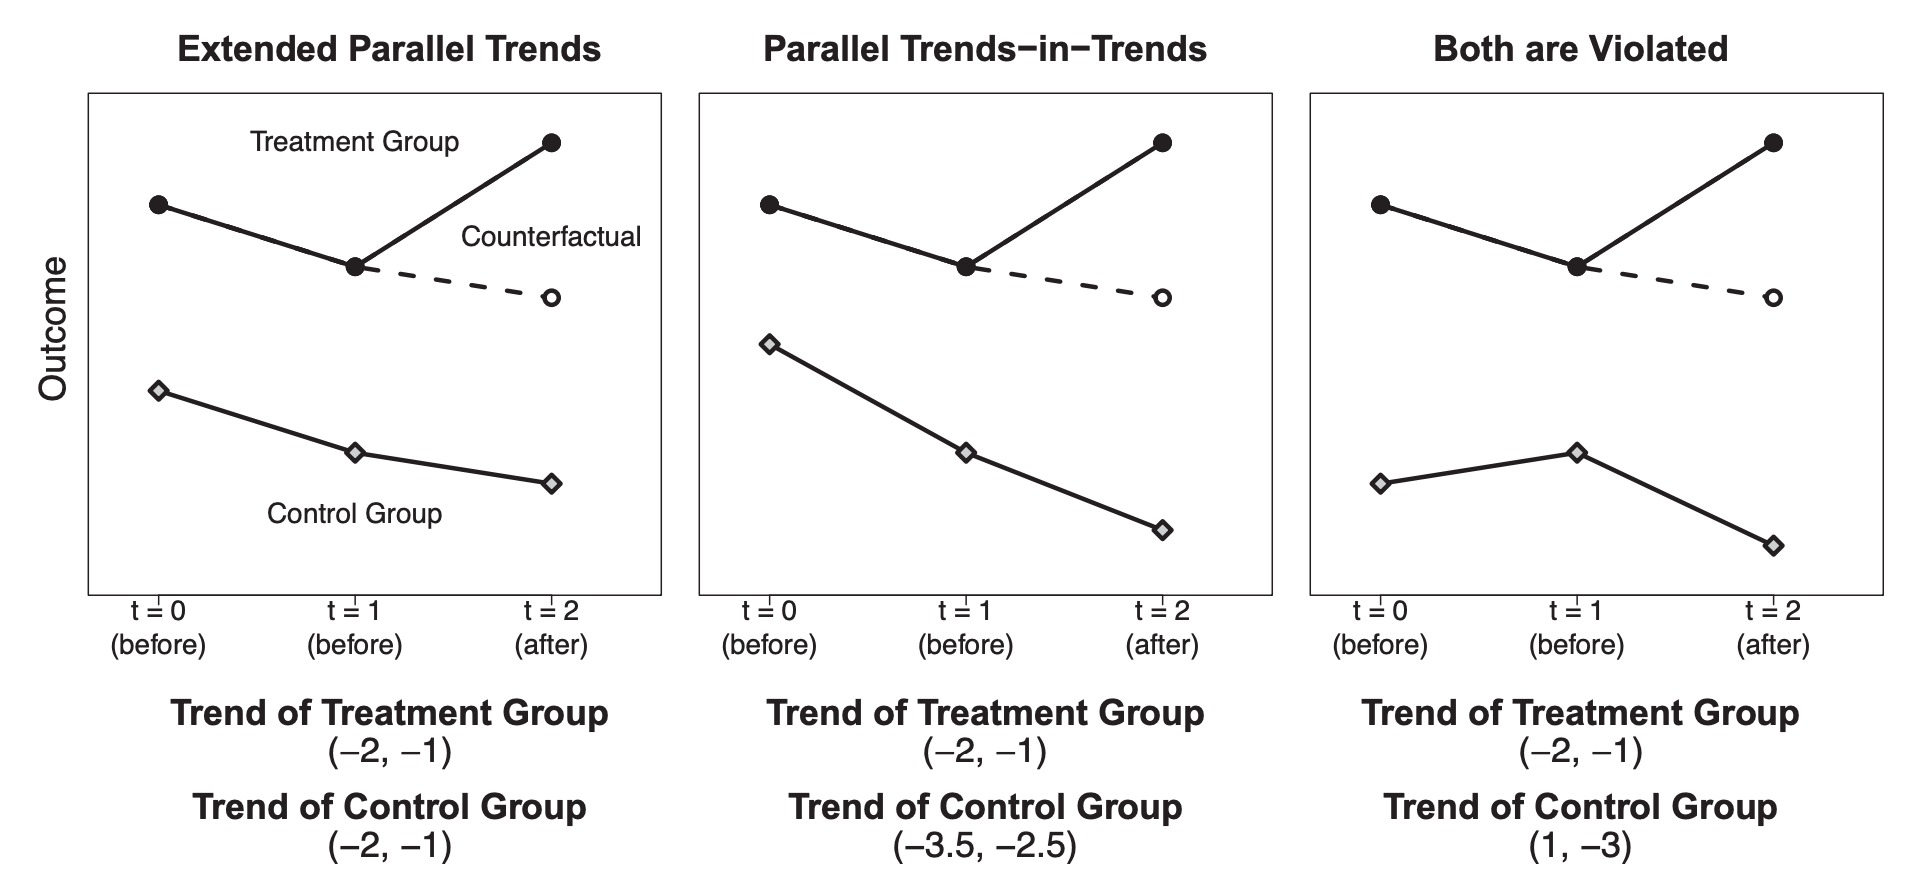
\includegraphics[width = \textwidth]{figures/ey_fig2}};
\node<3> at (.5,.5) {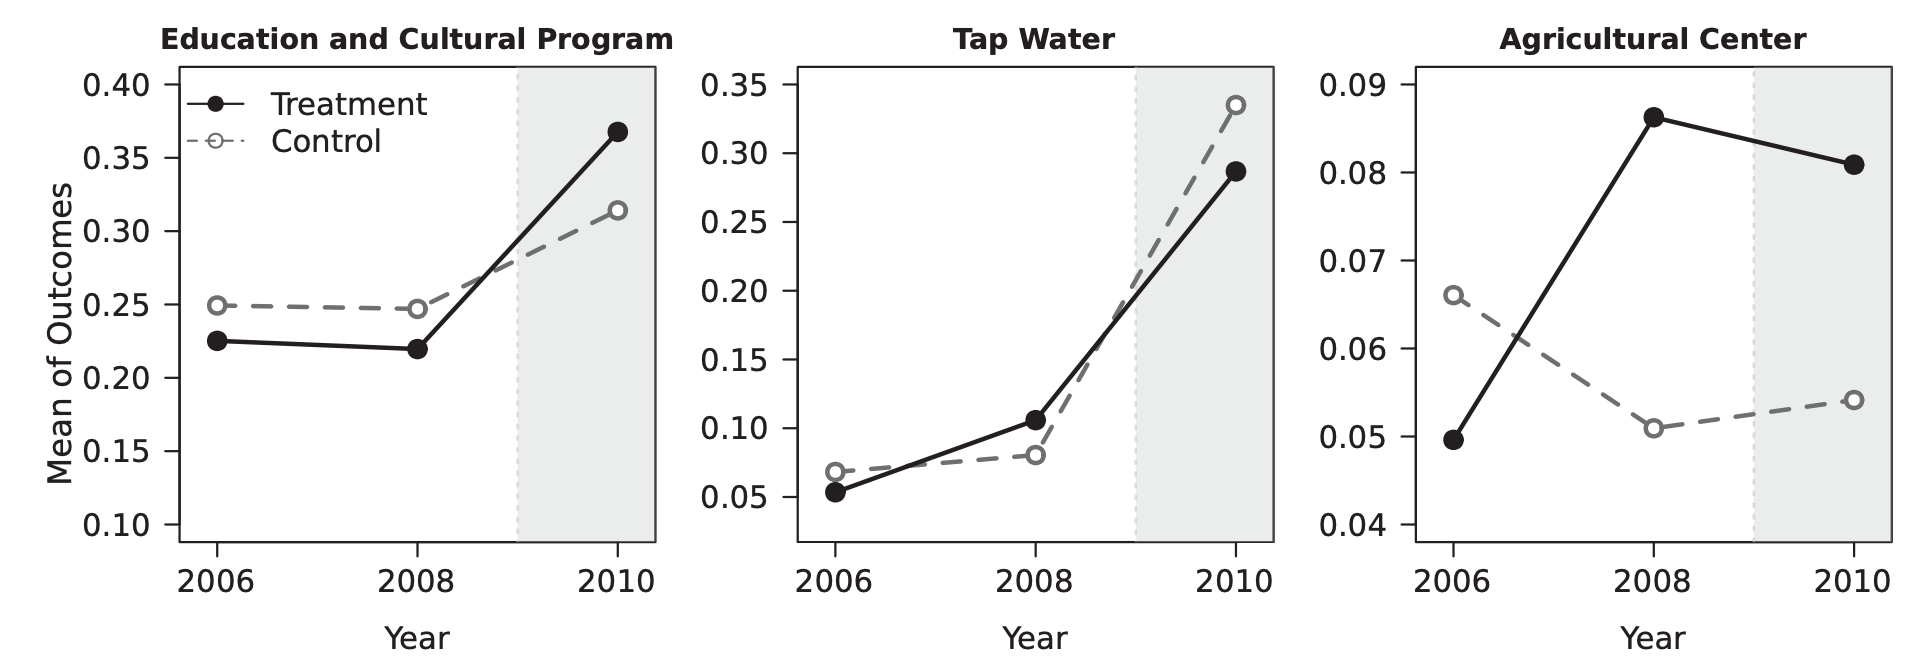
\includegraphics[width = \textwidth]{figures/ey_fig3}};
\end{tikzpicture}
\end{frame}

\section{Interrupted Time Series}

\begin{frame}[t]{Interrupted time series\footnote{Bernal, J. L., Cummins, S., \& Gasparrini, A. (2017). \bref{https://doi.org/10.1093/ije/dyw098}{Interrupted time series regression for the evaluation of public health interventions: A tutorial.} International Journal of Epidemiology, 46(1), 348-355.\\{}}} \pause \vskip .2in
You study one unit. It is untreated. Then it is treated. \vskip .2in \pause
\begin{center}
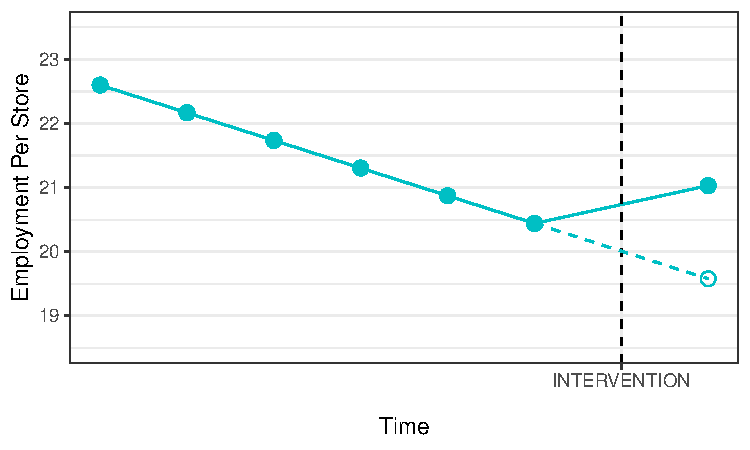
\includegraphics[width = .4\textwidth]{figures/parallel_trends_doubtful_4.pdf} \vskip .1in
\end{center}
\only<3-5>{In what settings does this work well?
\begin{itemize}
\item<4-5> When you have a strong pre-treatment trend to forecast $Y^0_t$
\item<5> When you don't have a comparable unit that is never treated
\end{itemize}
}
\only<6>{\bgray{Theoretical Estimand}\\$$\E(Y^1 - Y^0\mid T > t_\text{Intervention})$$}
\only<7-8>{\bgray{Identifying Assumption}
\begin{itemize}
\item<8> In the absence of the intervention,\\the pre-intervention trend in $Y^0$ would have continued
\end{itemize}}
\only<9->{Concrete steps:}
\begin{enumerate}
\item<10-> Learn a model on the pre-treatment period
\begin{itemize}
\item<11-> Evaluation metric: Forecast within the pre-treatment period
\end{itemize}
\item<12-> Forecast $Y^0$ for the post-treatment period
\end{enumerate}
\end{frame}

\begin{frame}[t]{Interrupted time series: When it becomes doubtful}
\includegraphics<2>[width = \textwidth]{figures/its_problem_1}
\includegraphics<3>[width = \textwidth]{figures/its_problem_2}
\includegraphics<4>[width = \textwidth]{figures/its_problem_3}
\includegraphics<5>[width = \textwidth]{figures/its_problem_4}
\includegraphics<6>[width = \textwidth]{figures/its_problem_5}
\end{frame}

\begin{frame}{Interrupted time series: Recap}
\begin{itemize}
\item ITS applies when treatment turns on at one time for all units
\item ITS requires a parametric model to extrapolate
\item ITS is most credible near the time when treatment turns on
\end{itemize}
\end{frame}

\begin{frame}{When to use each method}
\begin{itemize}\setlength\itemsep{.5em}\small
\item Difference in difference
\begin{itemize}\setlength\itemsep{.1em}\footnotesize
\item One unit becomes treated \hfill New Jersey
\item One unit never becomes treated \hfill Pennsylvania
\item The trends in $Y^0$ are parallel
\end{itemize}
\item Interrupted time series
\begin{itemize}\setlength\itemsep{.1em}\footnotesize
\item Everyone becomes treated at $X = c$\hfill New drug
\item You believe you can forecast $Y^0$\hfill Deaths would\\from $X < c$ to $X > c$\hfill have been stable
\end{itemize}
\end{itemize}
\end{frame}

\section{Regression Discontinuity}

\begin{frame}{Regression discontinuity\footnote{Cattaneo, M. D., \& Titiunik, R. (2022). \bref{https://doi.org/10.1146/annurev-economics-051520-021409}{Regression discontinuity designs.} Annual Review of Economics, 14, 821-851.}}
\begin{tikzpicture}[x = \textwidth, y = .8\textheight]
\node at (0,0) {};
\node at (1,1) {};
\node<2->[anchor = west] (fig) at (0,.5) {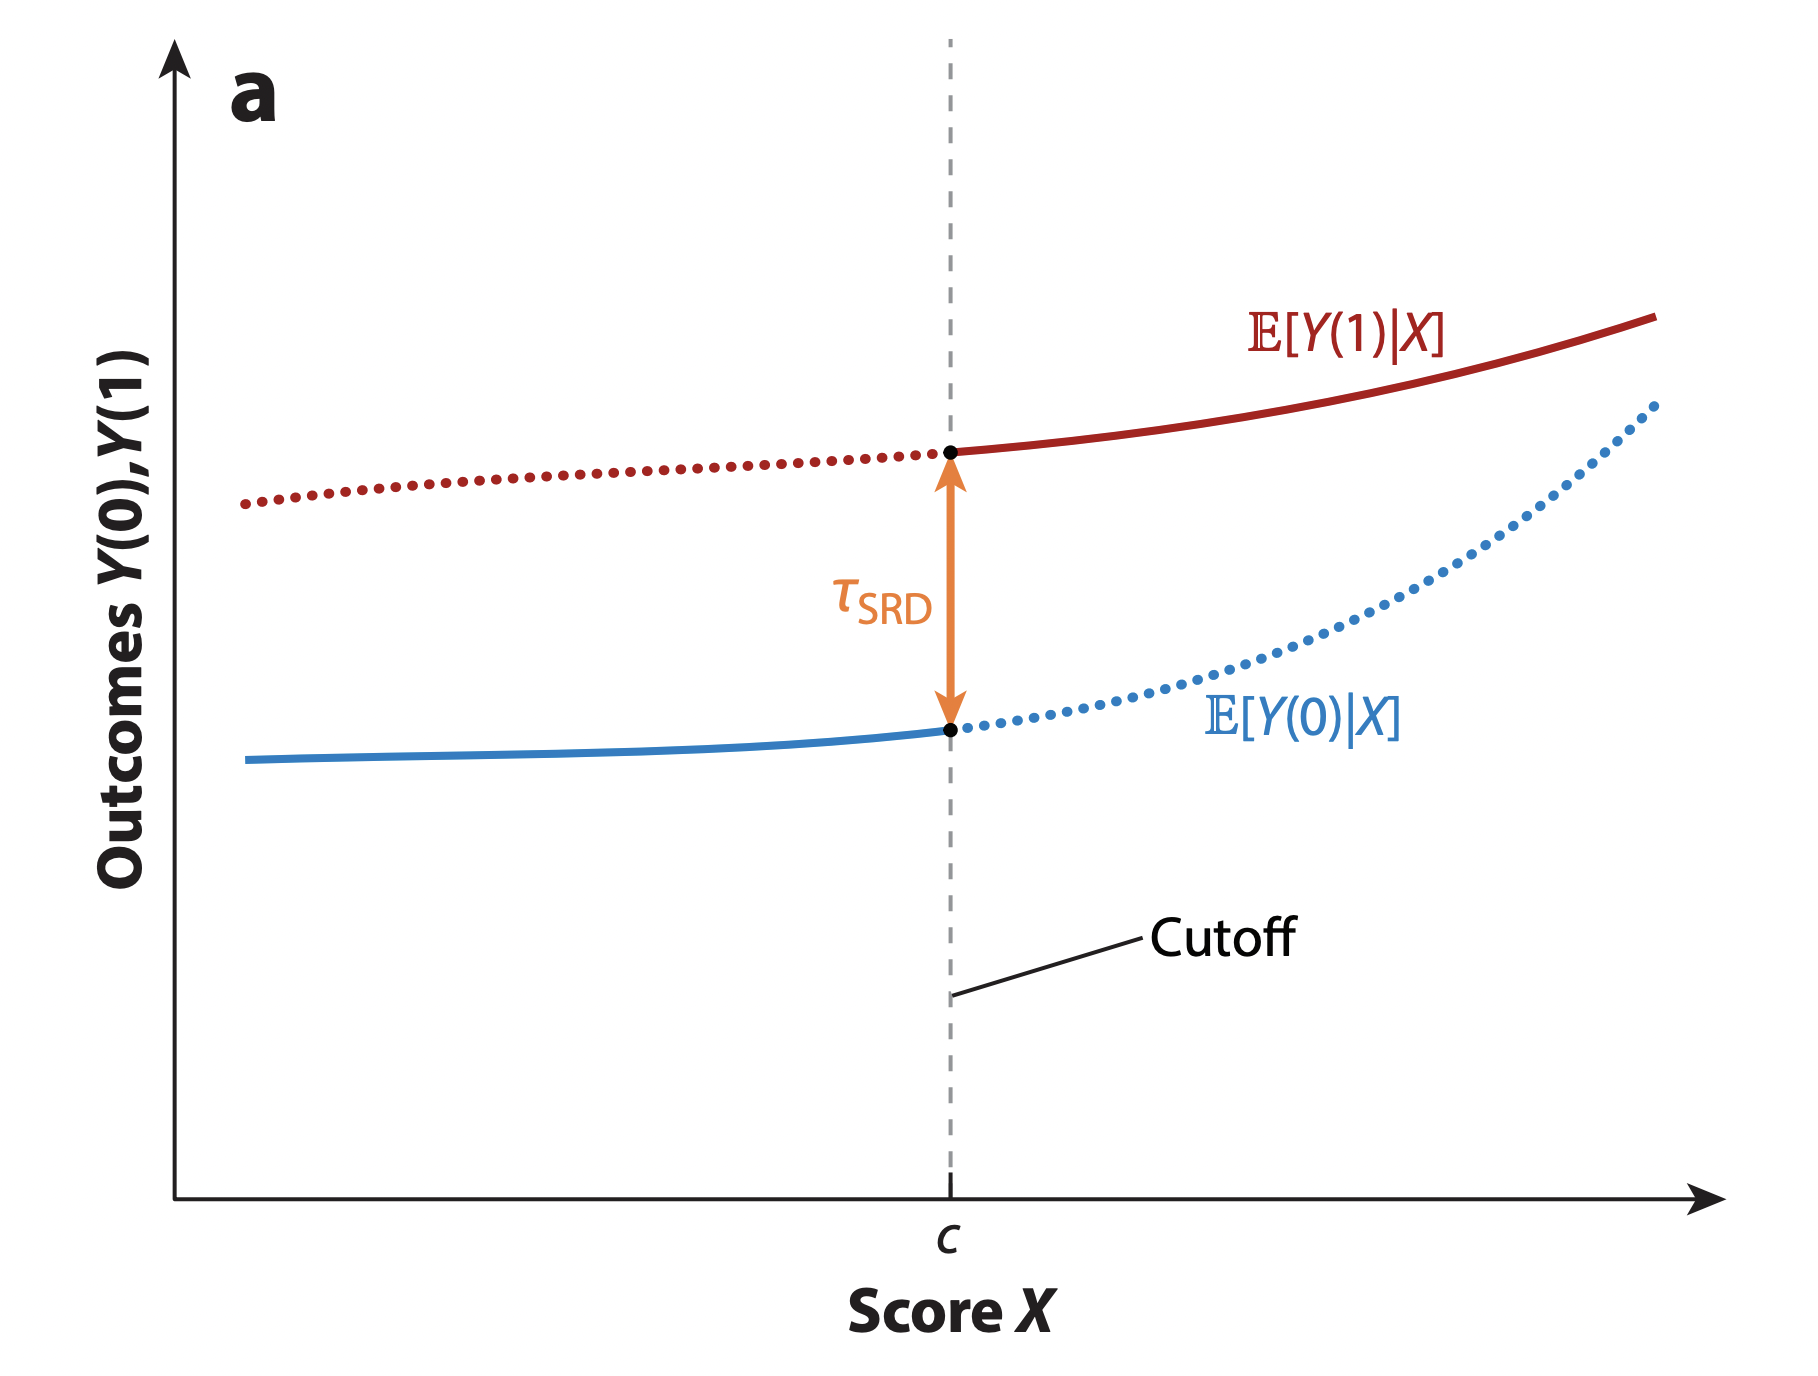
\includegraphics[width = .5\textwidth]{figures/ct_fig1a}};
\node<2->[anchor = south west, font = {\footnotesize\bf}] at (fig.north west) {Cattaneo \& Titiunik 2022 Fig 1a};
\node<3-6>[anchor = north west] at (.6, .9) {\bgray{Examples}};
\node<4-6>[anchor = north west, align = left, font = \small] at (.6, .8) {$X$ is PSAT test score\\$c$ is a score cutoff\\$A$ is National Merit Scholarship\\\begin{tiny}(\href{https://osf.io/tc5j7/download}{Thistlewaite \& Campbell 1960})\end{tiny}};
\node<5-6>[anchor = north west, align = left, font = \small] at (.6, .55) {$X$ is vote share\\$c$ is 50\%\\$A$ is winning the election\\\begin{tiny}(\href{https://imai.fas.harvard.edu/research/files/RD.pdf}{De la Cuesta \& Imai 2016})\end{tiny}};
\node<6>[anchor = north west, align = left, font = \small] at (.6, .3) {$X$ is date\\$c$ is 2am Nov 6 2022\\$A$ is hours of PM darkness};
\node<8-10>[anchor = north west, align = left] at (.6,.9) {\bgray{Theoretical Estimand}\\$\E(Y(1) - Y(0) \mid X = c)$};
\node<9-10>[anchor = north west, align = left] at (.6,.7) {\bgray{Empirical Estimand}\\$\text{lim}_{x\downarrow c}\E(Y\mid X = x)$\\\phantom{empirical}$-$\\$\text{lim}_{x\uparrow c}\E(Y\mid X = x)$};
\node<10>[anchor = north west, align = left] at (.6,.4) {\bgray{Identifying Assumptions}\\$\E(Y(1) \mid X = x)$ and\\$\E(Y(0) \mid X = x)$ are\\continuous at $x = c$\\{}\\and $f_X(x) > 0$ for $x$ near $c$};
\node<12->[anchor = north west, align = left] (p) at (.6,.85) {\bgray{Promises of RD}};
\node<13->[anchor = north west, align = left] (p1) at (p.south west) {--- Highly credible};
\node<14->[anchor = north west, align = left] (p2) at (p1.south west) {--- Easy to visualize};
\node<12->[anchor = north west, align = left] (d) at (.6,.5) {\bgray{Drawbacks of RD}};
\node<15->[anchor = north west, align = left] (d1) at (d.south west) {--- Local to $X = c$};
\node<16->[anchor = north west, align = left] (d2) at (d1.south west) {--- Sensitive to sorting};
\node<17->[anchor = north east, align = right] at (d2.south east) {(people moving\\strategically over\\the cutoff)};
\end{tikzpicture}
\end{frame}

\begin{frame}{When to use each method}
\begin{itemize}\setlength\itemsep{.5em}\small
\item Difference in difference
\begin{itemize}\setlength\itemsep{.1em}\footnotesize
\item One unit becomes treated \hfill New Jersey
\item One unit never becomes treated \hfill Pennsylvania
\item The trends in $Y^0$ are parallel
\end{itemize}
\item Interrupted time series
\begin{itemize}\setlength\itemsep{.1em}\footnotesize
\item Everyone becomes treated at $X = c$\hfill New drug
\item You believe you can forecast $Y^0$\hfill Deaths would\\from $X < c$ to $X > c$\hfill have been stable
\end{itemize}
\item Regression discontinuity
\begin{itemize}\setlength\itemsep{.1em}\footnotesize
\item Everyone becomes treated at $X = c$ \hfill Win the election
\item You want a local estimate\\$\E(Y^1 - Y^0 \mid X = c)$ at the cutoff\hfill Close elections
\item $Y^0$ and $Y^1$ are continuous at $X = c$
\end{itemize}
\end{itemize}
\end{frame}

\section{Synthetic Control}

\begin{frame}{Synthetic control\footnote{Abadie, A., Diamond, A., \& Hainmueller, J. (2010). \bref{http://www.jenshainmueller.de/Paper/ccs.pdf}{Synthetic control methods for comparative case studies: Estimating the effect of California’s tobacco control program.} Journal of the American Statistical Association, 105(490), 493-505.\\{}}} \pause
In 1988, California implemented a tobacco control program \pause
\begin{itemize}
\item New tax: 25 cents per pack \pause
\item Money earmarked for smoking-reduction programs
\end{itemize} \vskip .2in \pause
How much did it reduce CA cigarette sales in 1990? 1995? 2000?
\end{frame}

\begin{frame}{Synthetic control\footnote{Abadie, A., Diamond, A., \& Hainmueller, J. (2010). \bref{http://www.jenshainmueller.de/Paper/ccs.pdf}{Synthetic control methods for comparative case studies: Estimating the effect of California’s tobacco control program.} Journal of the American Statistical Association, 105(490), 493-505.\\{}}}

\begin{tikzpicture}[x = \textwidth, y = .6\textheight]
\node at (0,0) {};
\node at (1,1) {};
\node[anchor = west] at (0,.5) {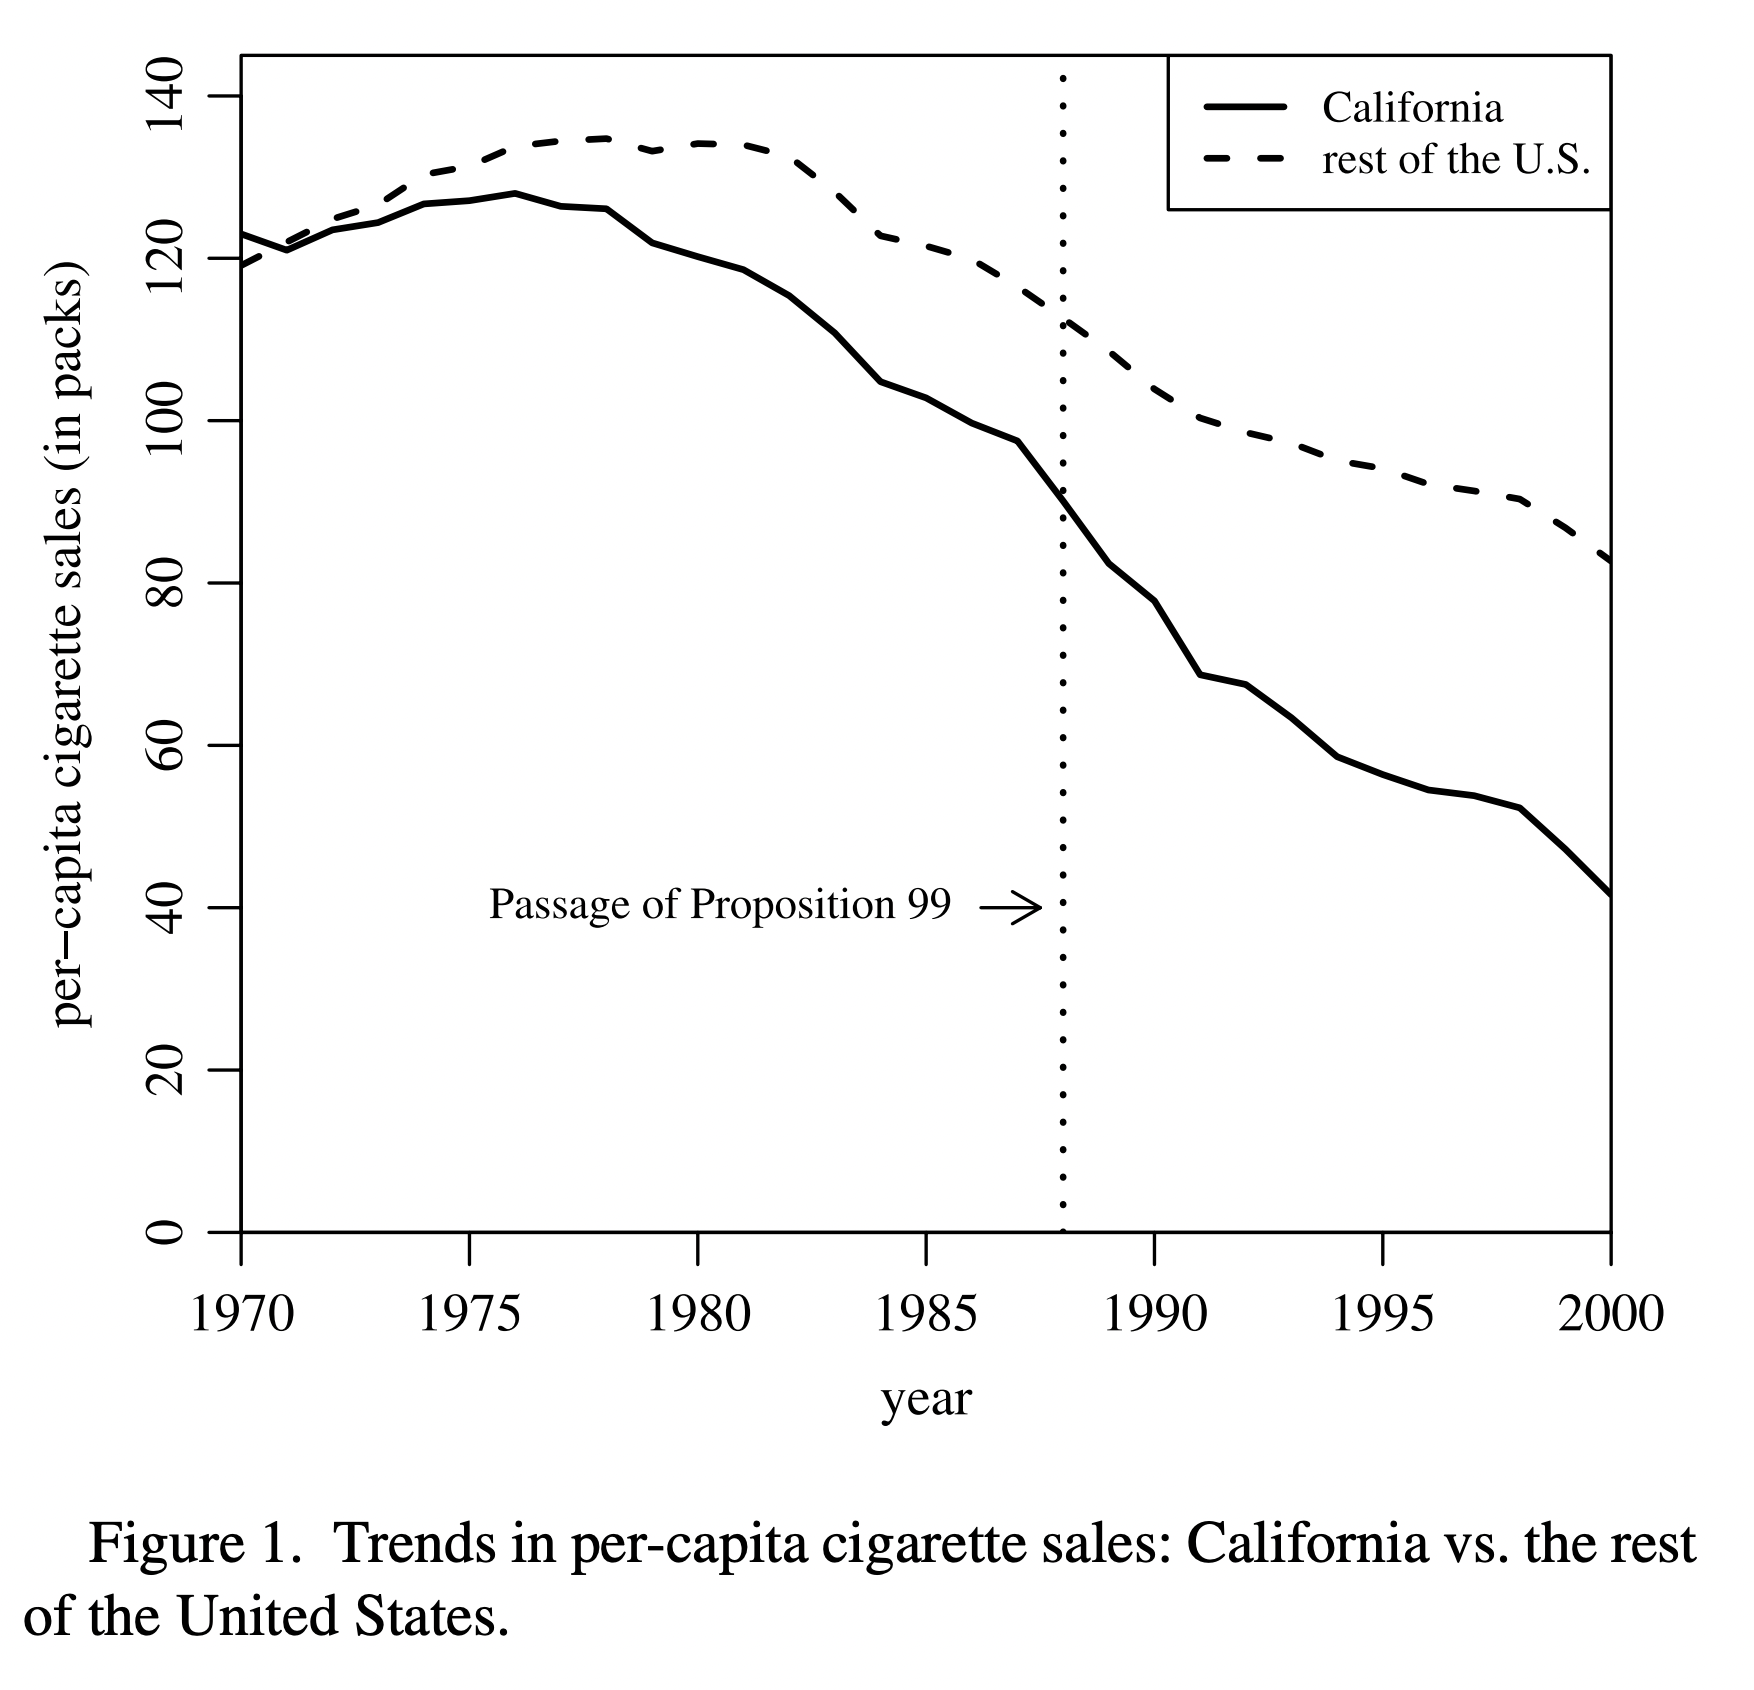
\includegraphics[height = .6\textheight]{figures/synth_fig1}};
\node[anchor = north west] at (.55,1) {Can't use RD};
\node[anchor = north west, font = \small] at (.55,.92) {--- Effect at 1988 not of interest};
\node[anchor = north west] at (.55,.8) {Can't use ITS};
\node[anchor = north west, font = \small] at (.55,.72) {--- Hard to extrapolate $Y^0$ trend};
\node[anchor = north west] at (.55,.6) {Can't use DID};
\node[anchor = north west, font = \small] at (.55,.52) {--- No other state like CA};
\node[anchor = north west, align = left] (idea) at (.65,.35) {Idea: Create a\\\bblue{synthetic CA}\\to estimate\\$Y^0_\text{CA,t}$ for $t \geq 1988$};
\draw[gray, thick] (idea.north east) -- (idea.north west) -- (idea.south west) -- (idea.south east);
\end{tikzpicture}

\end{frame}

\begin{frame}{Synthetic control\footnote{Abadie, A., Diamond, A., \& Hainmueller, J. (2010). \bref{http://www.jenshainmueller.de/Paper/ccs.pdf}{Synthetic control methods for comparative case studies: Estimating the effect of California’s tobacco control program.} Journal of the American Statistical Association, 105(490), 493-505.\\{}}}{Synthetic CA as a weighted average of other states}

\begin{center}
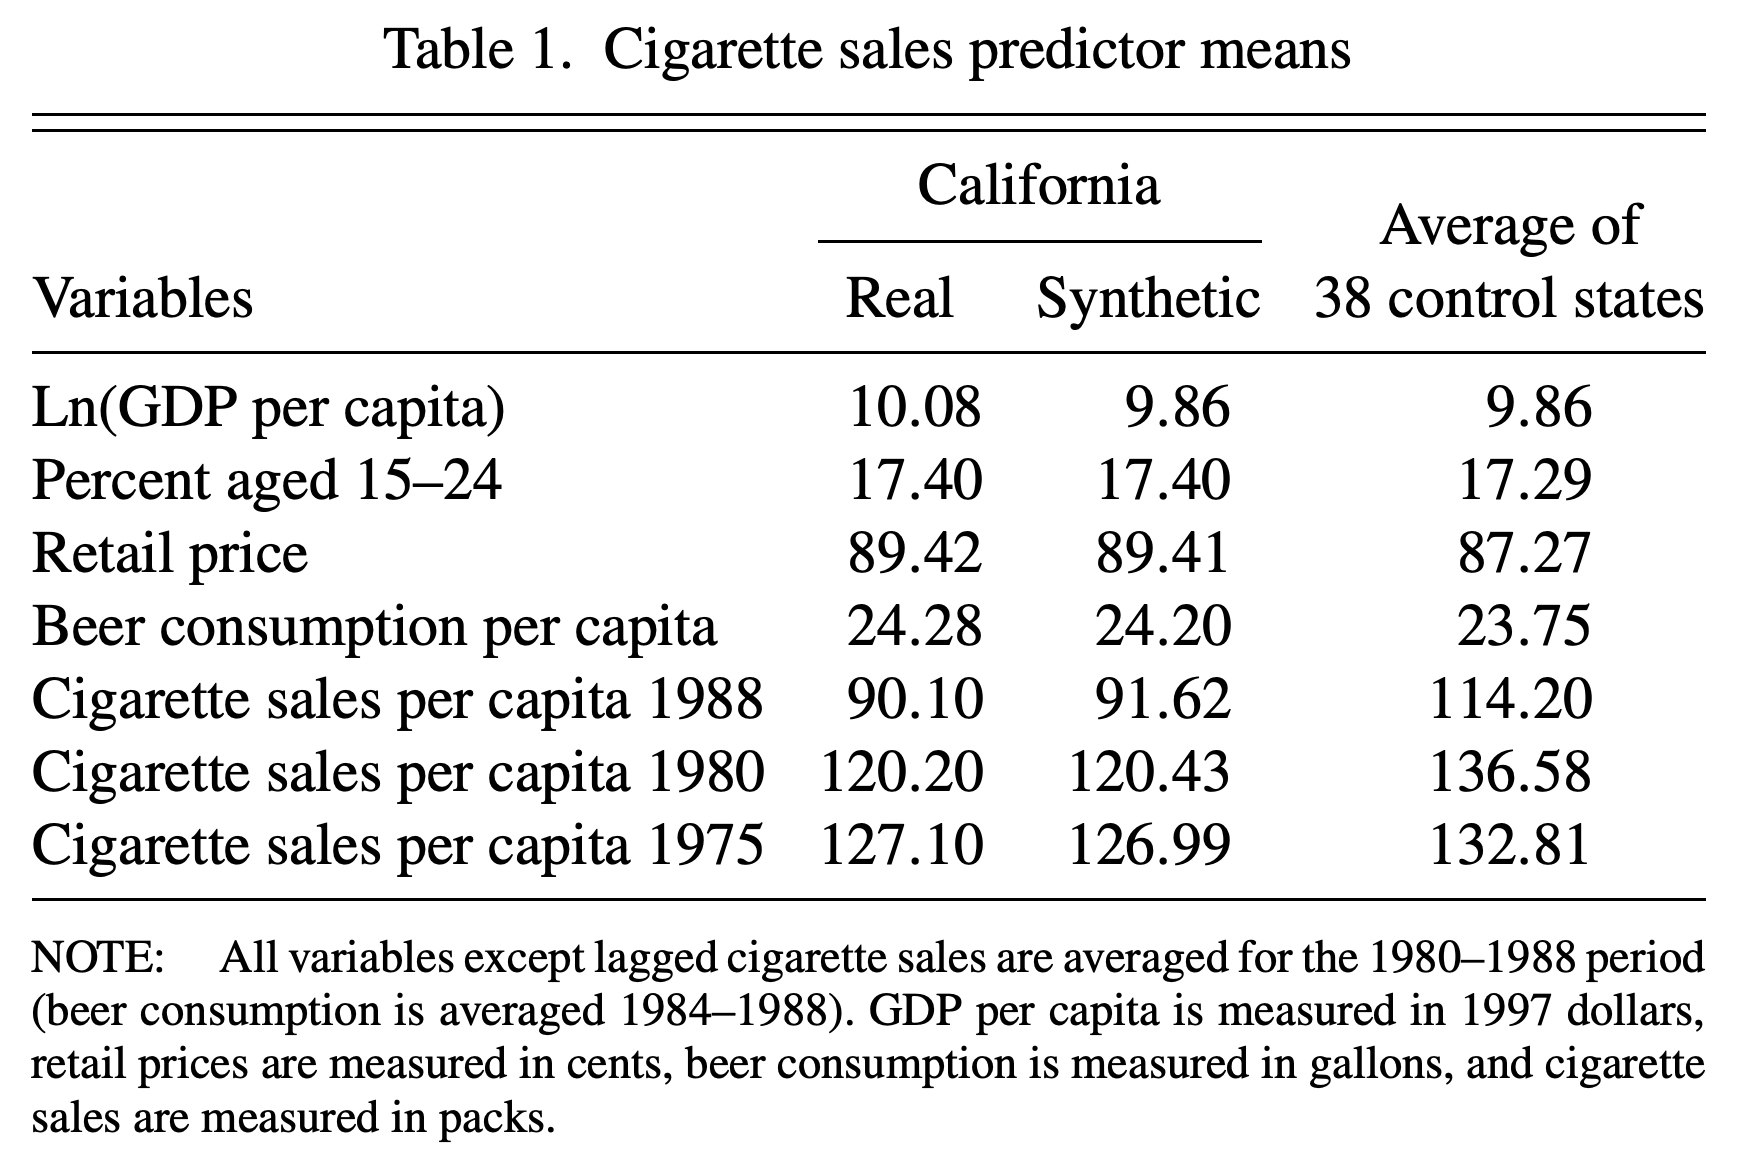
\includegraphics[height = .5\textheight]{figures/synth_tab1} \vskip .1in
\end{center}

\end{frame}

\begin{frame}{Synthetic control\footnote{Abadie, A., Diamond, A., \& Hainmueller, J. (2010). \bref{http://www.jenshainmueller.de/Paper/ccs.pdf}{Synthetic control methods for comparative case studies: Estimating the effect of California’s tobacco control program.} Journal of the American Statistical Association, 105(490), 493-505.\\{}}}{Synthetic CA as a weighted average of other states}

\begin{tabular}{rll}
Theoretical Estimand: & $\tau(t) = Y^1_{\text{CA},t}-Y^0_{\text{CA},t}$ & $t \geq 1988$ \\ \pause
\\
Empirical Estimand: & $\theta(t) = Y^1_{\text{CA},t}-Y^0_{\text{SyntheticCA},t}$ & $t \geq 1988$ \\ \pause
\\
Identifying Assumption: & $\underbrace{Y^0_{\text{CA},t}}_\text{Counterfactual} = \quad\underbrace{Y^0_{\text{SyntheticCA},t}}_\text{Factual}$ & $t \geq 1988$
\end{tabular}

\end{frame}

\begin{frame}{Synthetic control\footnote{Abadie, A., Diamond, A., \& Hainmueller, J. (2010). \bref{http://www.jenshainmueller.de/Paper/ccs.pdf}{Synthetic control methods for comparative case studies: Estimating the effect of California’s tobacco control program.} Journal of the American Statistical Association, 105(490), 493-505.\\{}}}

\centering
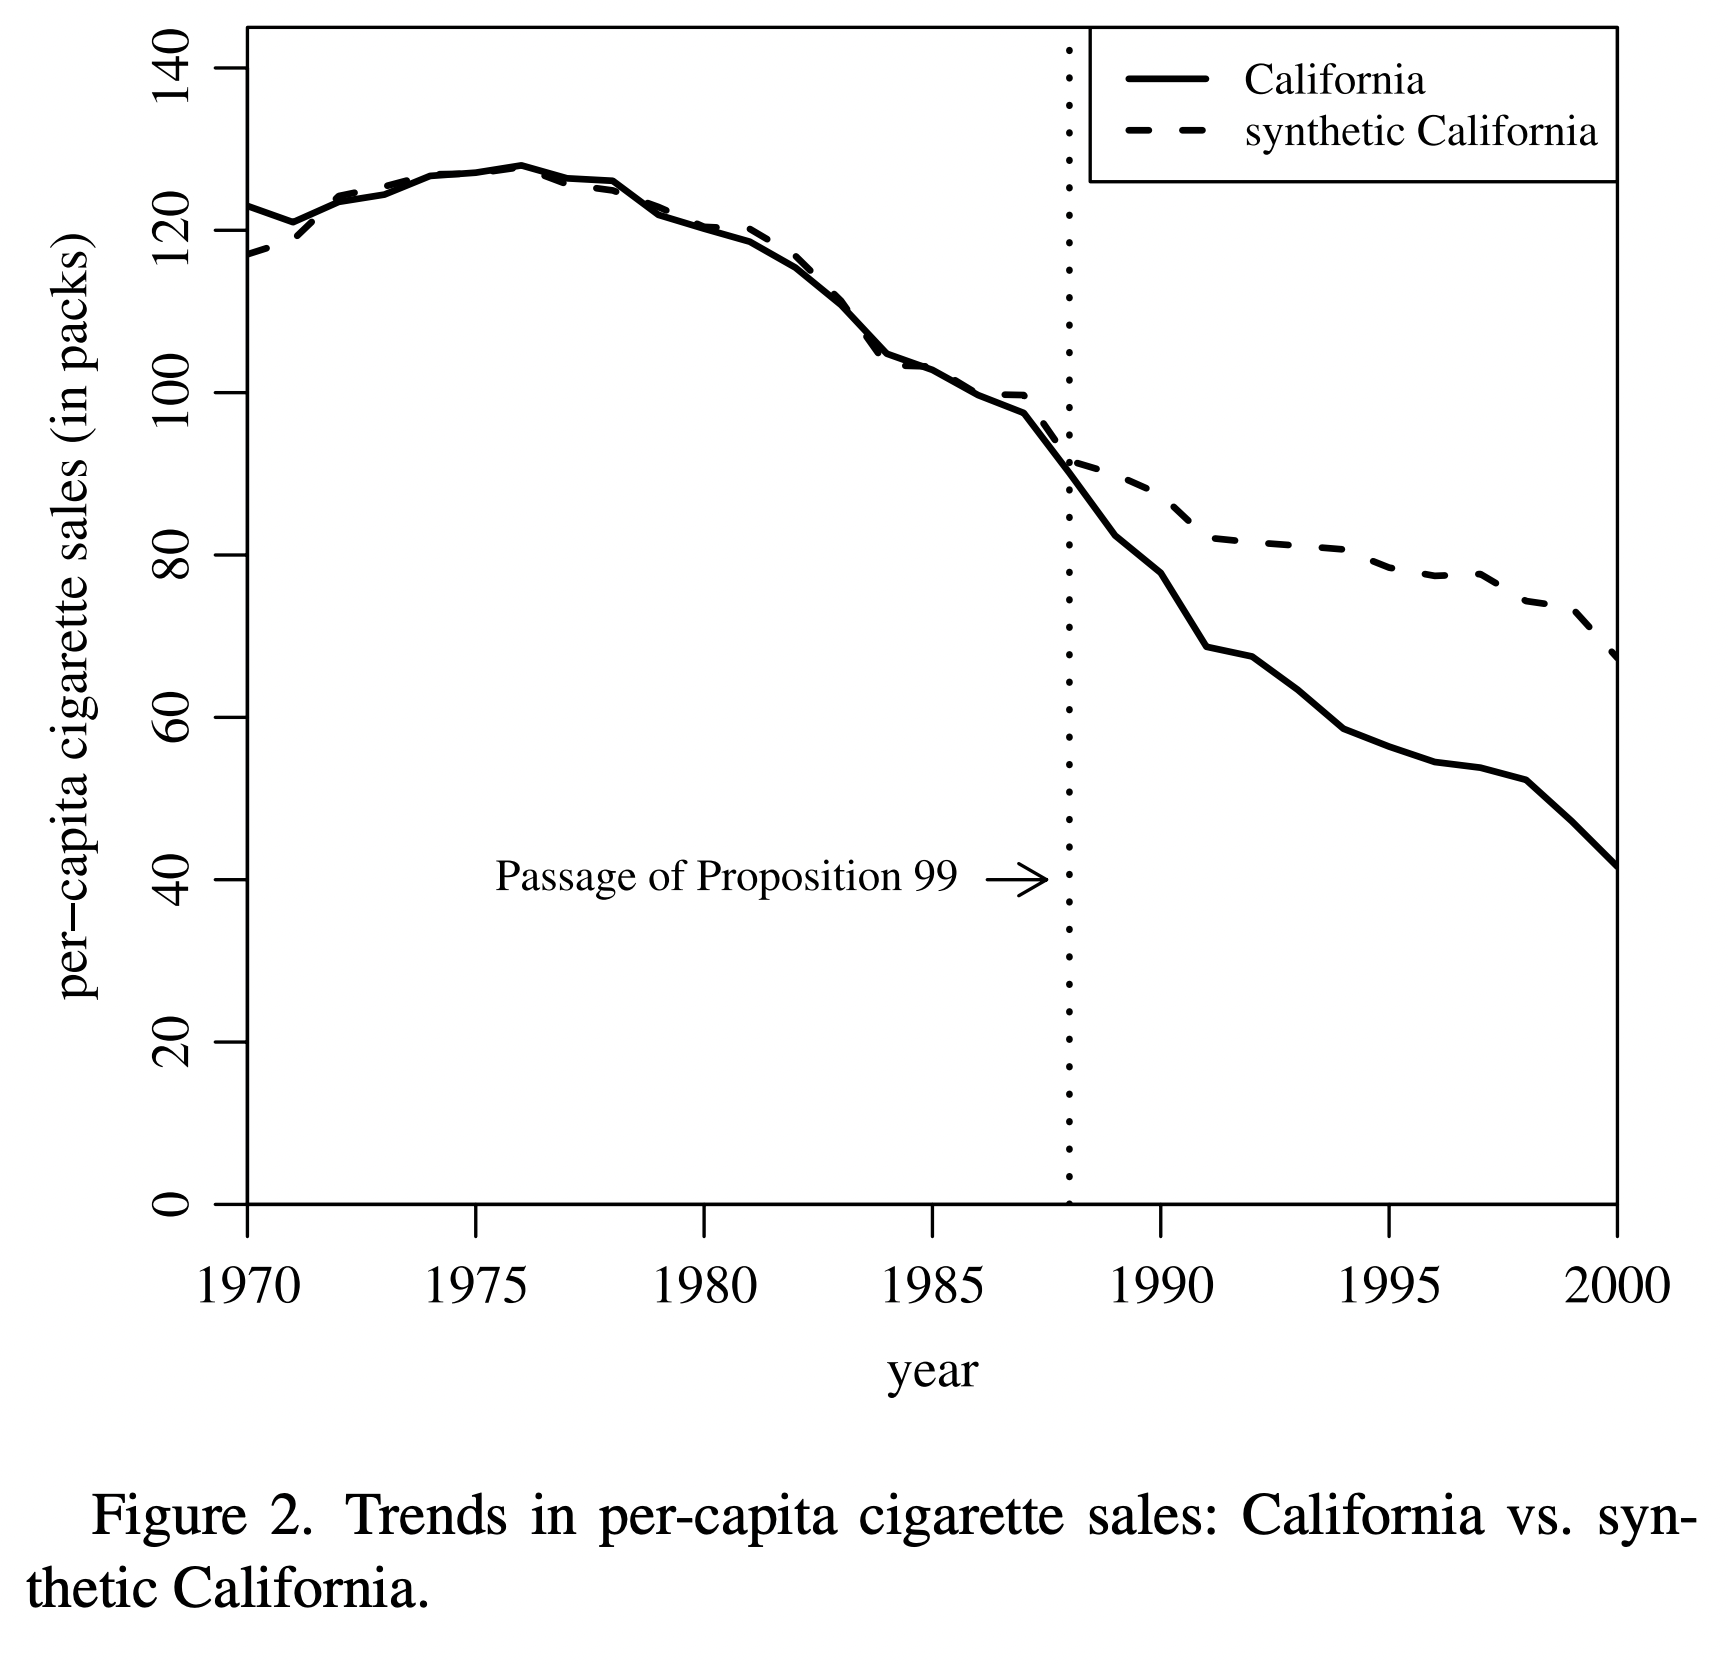
\includegraphics[height = .6\textheight]{figures/synth_fig2}

\end{frame}

\begin{frame}{When to use each method}
\begin{itemize}\setlength\itemsep{.5em}\small
\item Difference in difference
\begin{itemize}\setlength\itemsep{.1em}\footnotesize
\item One unit becomes treated \hfill New Jersey
\item One unit never becomes treated \hfill Pennsylvania
\item The trends in $Y^0$ are parallel
\end{itemize}
\item Interrupted time series
\begin{itemize}\setlength\itemsep{.1em}\footnotesize
\item Everyone becomes treated at $X = c$\hfill New drug
\item You believe you can forecast $Y^0$\hfill Deaths would\\from $X < c$ to $X > c$\hfill have been stable
\end{itemize}
\item Regression discontinuity
\begin{itemize}\setlength\itemsep{.1em}\footnotesize
\item Everyone becomes treated at $X = c$ \hfill Win the election
\item You want a local estimate\\$\E(Y^1 - Y^0 \mid X = c)$ at the cutoff\hfill Close elections
\item $Y^0$ and $Y^1$ are continuous at $X = c$
\end{itemize}
\item Synthetic control
\begin{itemize}\setlength\itemsep{.1em}\footnotesize
\item One unit becomes treated \hfill California
\item Many units are never treated \hfill Other states
\item You want to extrapolate far from the cutoff \hfill 1988$\rightarrow$2000
\end{itemize}
\end{itemize}
\end{frame}

\begin{frame}{Discussion}

\begin{itemize}
\item What data do you need to use the method?
\item What are the most likely limitations?
\item How would you generalize your method to settings where many units become treated, potentially at different time points (staggered adoption)?
\end{itemize}

\end{frame}

\goalsframe


\end{document}
